\documentclass[
	openany,
	% -- opções da classe memoir --
	12pt,				% tamanho da fonte
   % openright,
	%twoside,
    oneside,
    % para impressão em verso e anverso. Oposto a oneside
	a4paper,			% tamanho do papel. 
	english				% o último idioma é o principal do documento
	]{abntex2}

% ---
% Pacotes básicos 
% ---

\usepackage{fontspec}
\setmainfont{Arial}

\usepackage[utf8]{inputenc}		% Codificacao do documento (conversão automática dos acentos)
\usepackage{indentfirst}		% Indenta o primeiro parágrafo de cada seção.
\usepackage{color}				% Controle das cores
\usepackage{graphicx}			% Inclusão de gráficos
\usepackage{microtype} 			% para melhorias de justificação
\usepackage{multicol}			% multiplas colunas no texto
\usepackage{subcaption}
\usepackage{caption}
\usepackage{float}
\usepackage{amsmath}
\usepackage{amssymb}
\usepackage{amsthm}
\usepackage{lipsum}
\usepackage{blindtext}
\usepackage{lscape}
\usepackage{booktabs}
\usepackage{hyperref}
\usepackage{comment}
\usepackage{caption}
\usepackage{subcaption}

%\usepackage[square,sort&compress,comma,numbers,nonamebreak,longnamesfirst]{natbib}

% ---
% ---
% Pacotes de citações
% ---
\usepackage[brazilian]{backref}	 % Paginas com as citações na bibl
\usepackage[alf]{abntex2cite}	% Citações padrão ABNT



% --- 
% CONFIGURAÇÕES DE PACOTES
% --- 

% ---
% Configurações do pacote backref
% Usado sem a opção hyperpageref de backref
\renewcommand{\backrefpagesname}{Citado na(s) página(s):~}
% Texto padrão antes do número das páginas
\renewcommand{\backref}{}
% Define os textos da citação
\renewcommand*{\backrefalt}[4]{
	\ifcase #1 %
		Nenhuma citação no texto.%
	\or
		Citado na página #2.%
	\else
		Citado #1 vezes nas páginas #2.%
	\fi}%
% ---

% ---
% Informações de dados para CAPA e FOLHA DE ROSTO
% ---
\titulo{Modelos Computacionais para a Simulação e Análise da Detecção de Ondas Gravitacionais.}
\autor{Gerson Rodrigues Santos}
\local{Recife}
\data{2018}
\orientador{Prof. Tiago A. E. Ferreira}
\coorientador{Prof. Antônio de Pádua Santos}


\instituicao{%
	Universidade Federal Rural de Pernambuco -- UFRPE
  	\par
  	Departamento de Estatística e Informática
    \par
  	Mestrado em Informática Aplicada
}

\tipotrabalho{Trabalho de Conclusão de Curso}
% O preambulo deve conter o tipo do trabalho, o objetivo, 
% o nome da instituição e a área de concentração 
\preambulo{Projeto de Dissertação apresentado ao Curso de Mestrado em Informática Aplicada da Universidade Federal Rural de Pernambuco como requisito parcial para conclusão do Curso.}
% ---


% ---
% Configurações de aparência do PDF final

% alterando o aspecto da cor azul
\definecolor{blue}{RGB}{41,5,195}

% informações do PDF
\makeatletter
\hypersetup{
     	%pagebackref=true,
		pdftitle={\@title}, 
		pdfauthor={\@author},
    	pdfsubject={\imprimirpreambulo},
	    pdfcreator={LaTeX with abnTeX2},
		colorlinks=true,       		% false: boxed links; true: colored links
    	linkcolor=blue,          	% color of internal links
    	citecolor=blue,        		% color of links to bibliography
    	filecolor=magenta,      		% color of file links
		urlcolor=blue,
		bookmarksdepth=4
}
\def\MT@is@composite#1#2\relax{%
  \ifx\\#2\\\else
    \expandafter\def\expandafter\MT@char\expandafter{\csname\expandafter
                    \string\csname\MT@encoding\endcsname
                    \MT@detokenize@n{#1}-\MT@detokenize@n{#2}\endcsname}%
    % 3 lines added:
    \ifx\UnicodeEncodingName\@undefined\else
      \expandafter\expandafter\expandafter\MT@is@uni@comp\MT@char\iffontchar\else\fi\relax
    \fi
    \expandafter\expandafter\expandafter\MT@is@letter\MT@char\relax\relax
    \ifnum\MT@char@ < \z@
      \ifMT@xunicode
        \edef\MT@char{\MT@exp@two@c\MT@strip@prefix\meaning\MT@char>\relax}%
          \expandafter\MT@exp@two@c\expandafter\MT@is@charx\expandafter
            \MT@char\MT@charxstring\relax\relax\relax\relax\relax
      \fi
    \fi
  \fi
}
% new:
\def\MT@is@uni@comp#1\iffontchar#2\else#3\fi\relax{%
  \ifx\\#2\\\else\edef\MT@char{\iffontchar#2\fi}\fi
}
\makeatother
% --- 

% --- 
% Espaçamentos entre linhas e parágrafos 
% --- 

% O tamanho do parágrafo é dado por:
\setlength{\parindent}{1.3cm}

% Controle do espaçamento entre um parágrafo e outro:
\setlength{\parskip}{0.2cm}  % tente também \onelineskip

% ---
% compila o indice
% ---
\makeindex
% ---

% ----
% Início do documento
% ----
\begin{document}

% Seleciona o idioma do documento (conforme pacotes do babel)
% \selectlanguage{english}
\selectlanguage{brazil}

% Retira espaço extra obsoleto entre as frases.
\frenchspacing 

% ----------------------------------------------------------
% ELEMENTOS PRÉ-TEXTUAIS
% ----------------------------------------------------------
% \pretextual
%\begin{figure}[h]
%\centering % este comando é usado para centralizar a figura
%
\includegraphics[width=7cm]{figuras/logo_ufrpe_horizontal.png}\\
%\end{figure}

% \begin{figure}[ht]
% \centering
% \begin{minipage}[b]{0.45\textwidth}
% 
\includegraphics[height=3cm]{figuras/logo_ufrpe_horizontal.png}
% \end{minipage}
% \qquad
% \begin{minipage}[b]{0.45\textwidth}
% \includegraphics[height=2.5cm]{figuras/logo_bsi.pdf}
% \end{minipage}
% \end{figure}

%\begin{minipage}[t]{1\textwidth}
	\begin{figure}[ht]
		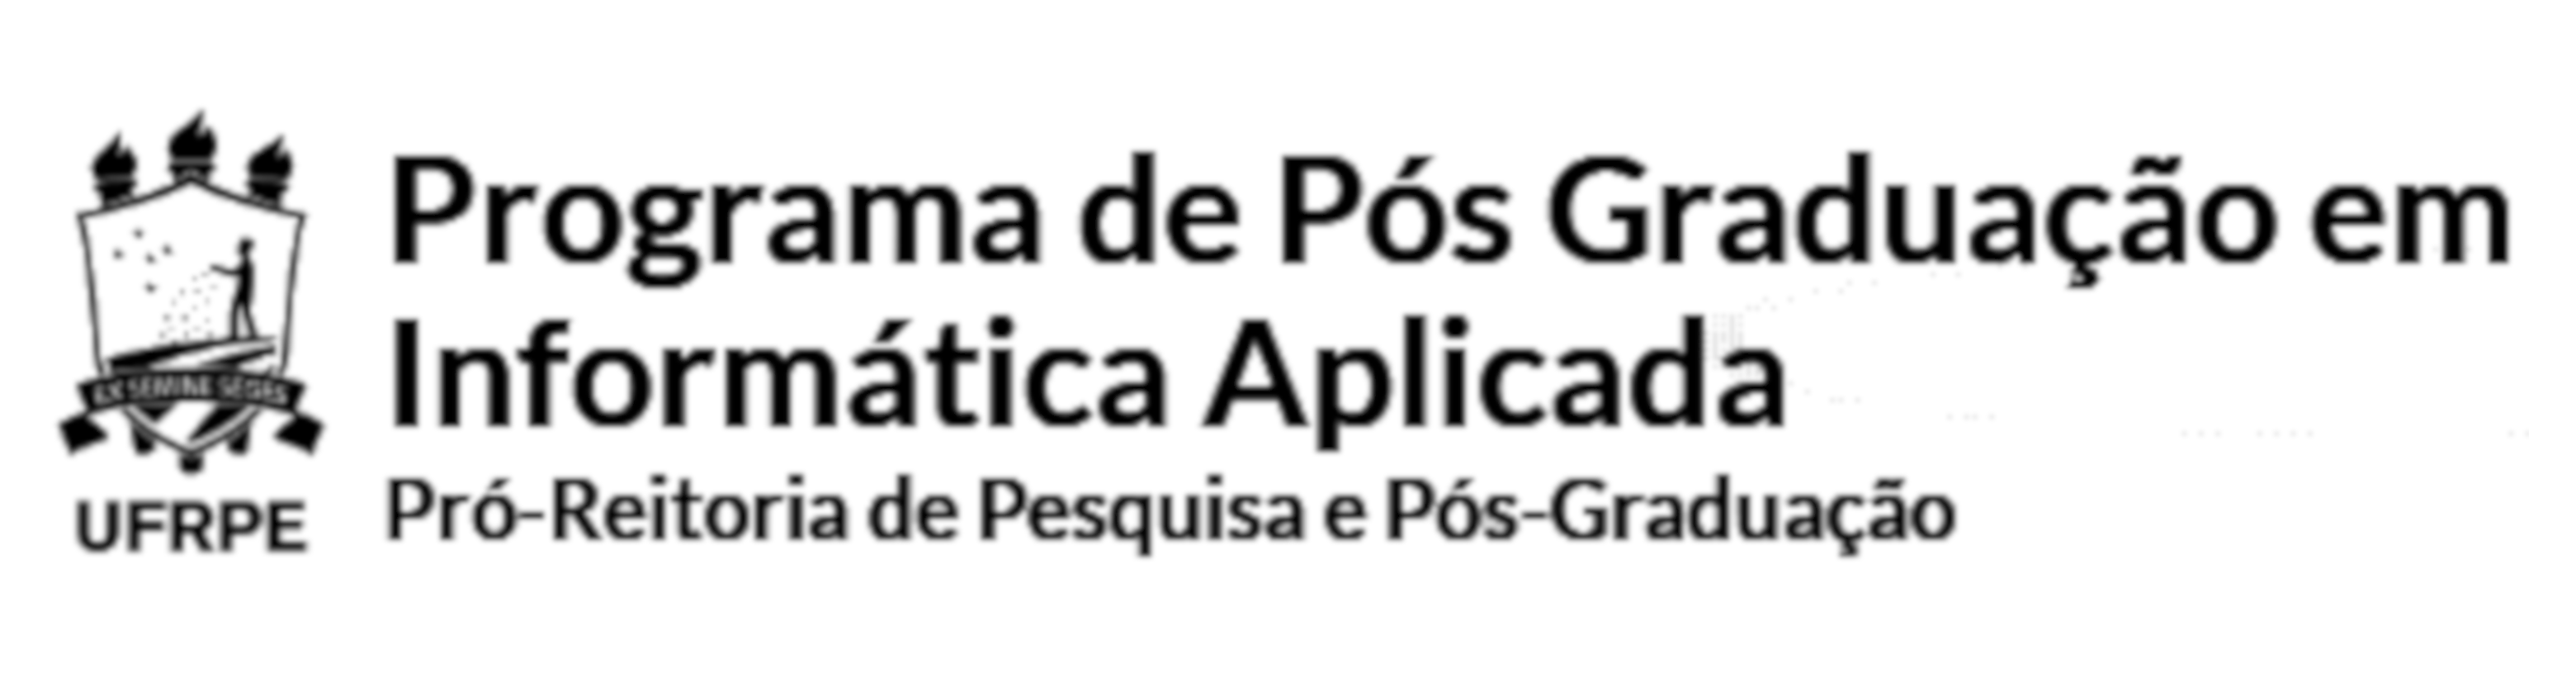
\includegraphics[height=4cm]{figuras/logo_ppgia.png}
	\end{figure}
%\end{minipage}

% ---
% Capa
% ---
\imprimircapa
% ---
% ---
% Folha de rosto
% (o * indica que haverá a ficha bibliográfica)
% ---
\imprimirfolhaderosto
% ---

% dedicatoria
\begin{dedicatoria}
   \vspace*{\fill}
   \centering
   \noindent
   \textit{À \ldots\\} \vspace*{\fill}
\end{dedicatoria}

% agradecimentos
\begin{agradecimentos}
Agradeço aos meus orientadores e amigos, o Prof. Dr. Tiago Alessandro Espinola Ferreira e o Prof. Dr. Antônio de Pádua Santos , por terem confiado e apostado em meu trabalho, por serem os guias neste caminho percorrido e pelo exemplo de pessoas comprometidas com o trabalho.
\end{agradecimentos}

% epigrafe
\begin{epigrafe}
    \vspace*{\fill}
	\begin{flushright}
		\textit{``A Ciência não tem medo de assumir a sua ignorância, de assumir os limites do que podemos explicar e com isso avançar. Quem se contenta com explicações fechadas e definitivas, ficam com elas. Nós, ficamos com eventos cósmicos capazes de mudar o universo.'' \\
		(Albert Einstein)}
	\end{flushright}
\end{epigrafe}

% resumo e abstract
\setlength{\absparsep}{18pt} % ajusta o espaçamento dos parágrafos do resumo
\begin{resumo}
 
A astronomia de ondas gravitacionais colocou em movimento uma revolução científica. Para aumentar ainda mais o alcance científico desse campo emergente, há uma necessidade premente de aumentar a profundidade e a velocidade dos algoritmos de ondas gravitacionais que permitiram essas descobertas inovadoras. Para contribuir com esse esforço, pretende-se criar  um novo método altamente escalonável para processamento de sinais de séries temporais end-to-end, baseado em um sistema de redes neurais, para classificação de sinais em fluxos de dados de séries temporais altamente ruidosos. Demonstrando um novo esquema de treinamento com níveis de ruído gradualmente crescentes. Validar a aplicação deste método para a detecção de ondas gravitacionais a partir de fusões binárias de buracos negros. E espera-se que este método supere significativamente as técnicas convencionais de aprendizado de máquina, obtendo desempenho similar em comparação com a filtragem combinada, sendo várias vezes mais rápido, permitindo o processamento em tempo real de grandes volumes de dados brutos com recursos mínimos. Mais importante, o método proposto amplia a gama de sinais de ondas gravitacionais que podem ser detectados com detectores de ondas gravitacionais terrestres. Essa estrutura aproveita os avanços recentes em algoritmos de inteligência artificial e em arquiteturas de hardware emergentes, como GPUs otimizadas para aprendizado de maquina, para facilitar as pesquisas em tempo real de fontes de ondas gravitacionais e suas contrapartes eletromagnéticas e astro-partícula.

 \textbf{Palavras-chave}: Ondas Gravitacionais, Aprendizado de Maquina, Learning Machine, Buracos Negros, Ruídos.
\end{resumo}


\begin{resumo}[Abstract]
 \begin{otherlanguage*}{english}
  
Gravitational wave astronomy has set in motion a scientific revolution. To further increase the scientific reach of this emerging field, there is a pressing need to increase the depth and speed of gravitational wave algorithms that have allowed these breakthrough discoveries. To contribute to this effort, we intend to create a new highly scalable method for processing end-to-end time series signals based on a neural network system for signal classification in highly noisy time series data flows. Demonstrating a new training scheme with gradually increasing noise levels. Validate the application of this method for the detection of gravitational waves from binary black hole fusions. And this method is expected to significantly outperform conventional machine learning techniques, achieving similar performance compared to combined filtering, which is several times faster, allowing real-time processing of large volumes of raw data with minimal features. More importantly, the proposed method extends the range of gravitational wave signals that can be detected with terrestrial gravitational wave detectors. This framework leverages recent advances in artificial intelligence algorithms and emerging hardware architectures such as machine-optimized GPUs to facilitate real-time searches of gravitational wave sources and their astro-particle and electromagnetic counterparts.
   \textbf{Keywords}:  Gravitational Waves, Machine Learning, Learning Machine, Black Holes, Noise.
 \end{otherlanguage*}
\end{resumo}

% ---
% inserir lista de ilustrações
% ---
\pdfbookmark[0]{\listfigurename}{lof}
\listoffigures
\cleardoublepage
% ---

% ---
% inserir lista de tabelas
% ---
\pdfbookmark[0]{\listtablename}{lot}
\listoftables*
\cleardoublepage
% ---

% ---
% inserir lista de abreviaturas e siglas
% ---
\begin{siglas}
  \item[RNA] Rede Neural Artificial	
  \item[GW] Gravitational Wave
  \item[...] \ldots
\end{siglas}
% ---

% ---
% inserir o sumario
% ---
\pdfbookmark[0]{\contentsname}{toc}
\tableofcontents*
\cleardoublepage
% ---



% ----------------------------------------------------------
% ELEMENTOS TEXTUAIS
% ----------------------------------------------------------
\textual

% ----------------------------------------------------------
% inclusao das secoes do texto
% ----------------------------------------------------------
\chapter{Introdução}
A maneira que temos de observar a natureza e o universo sempre dependeu de instrumentos, microscópios trouxeram a noção de que micro-organismos extremamente pequenos existiam, nos permitiram descobrir as bactérias, as formas de vida mais comuns do planeta, telescópios nos deram habilidades de observar o sistema solar descobrir as órbitas dos planetas e formular a noção de gravidade de Newton \cite{newton1687philosophiae}. 

Mas nem sempre essas descobertas aconteceram de propósito. Em 1930, o físico Karl Jansky foi encarregado de melhorar os sinais de rádio que cruzavam os oceanos com telégrafos e chamadas de telefone, para detectar de onde vinham as ondas de rádio que atrapalhavam a chamada com estática. Jansky construiu uma antena giratória que podia apontar para todas as direções. Foi quando ele descobriu ondas de rádio vindas de tempestades de raios próximas e distantes e uma terceira fonte de rádio no céu. O sinal ficava mais forte a cada 23 horas e 56 minutos, o tempo que as estrelas levam para percorrer o céu, o nosso dia sideral \cite{singh2010big}. 

O ponto que ele descobriu, era o centro da nossa Via Láctea, com a maior parte dos sinais de rádio vindos da constelação de sagitário. De alguma forma o universo estava cheio de fontes de ondas de rádio, uma descoberta por acaso, feita sem querer por alguém que estava preparado para entender o que havia encontrado, uma serendipidade. 
Assim como o sol emite radiação eletromagnética na forma de ondas de luz. Também emite frequências maior e menor, como rádio. Com apenas 26 anos, Jansky publicou o trabalho que inaugurou a radioastronomia, a observação do universo com os radiotelescópios, que nos permite ver, de explosões aos bips de pulsares \cite{jansky1932directional}. Como ver em outras ondas além da luz nos mostra novos fenômenos, observações de raio-x, por exemplo, mostram buracos negros rasgando as estrelas \cite{200814}, os quasares, em quanto a radiação infravermelha atravessa a Via Láctea e nos mostra o que tem por trás dela. 

E o que a descoberta da radioastronomia teve de serendipidade, a descoberta das ondas gravitacionais (Gravitational wave) (GW) teve de proposital. Começando por Einstein. Em 1915, quando ele adicionou a gravidade à teoria da relatividade, Publicando a "Teoria da Relatividade Geral" \cite{albert1920realtivity}, Einstein concluiu que a gravidade não era uma força, mas sim a deformação do espaço tempo, e essa deformação do espaço deveria viajar pelo universo como uma onda, viajando na velocidade da luz, mas isso só havia sido observado indiretamente. 

Por volta de 1960, descobertas astronômicas (quasares, pulsares, radiação cósmica de fundo) e novos experimentos impulsionaram a relatividade geral, para a linha de frente. Neste período foi descoberto a diminuição no período orbital do pulsar binário Hulse-Taylor em uma taxa consistente com a predição da relatividade geral da perda de energia por ondas gravitacionais \cite{weisberg2004relativistic}, e essa havia sido a primeira detecção indireta de ondas gravitacionais da historia da ciência, havia, por que agora, observamos pela primeira vez, dois buracos negros se fundindo e liberando uma energia 10 vezes maior do que a emissão de luz por todas as galáxias do universo observável. 

Pra isso precisamos do Observatório de Ondas Gravitacionais por Interferometria a Laser (Advanced Laser Interferometer Gravitational Wave Observatory) (aLIGO) \cite{PhysRevLett.116.131103,0264-9381-32-7-074001}, que recentemente, até o momento, tem anunciado a detecção de ondas gravitacionais a partir de medidas de uma série de eventos cósmicos que envolvem colapso de sistemas binários formados por objetos compactos tais como buracos negros \cite{abbott2016observation,ligo2016gw151226,scientific2017gw170104,abbott2017gw170814}, e estrelas de nêutrons \cite{abbott2017gw170817}, que são consistentes com as previsões gerais de relatividade de Einstein.

O observatório tem dois centros, com formato em L um posicionado em Washington e outro em Louisiana nos Estados Unidos, na quina desse L um espelho divide um feixe de laser em duas partes, que percorrem, cada uma, um dos tubos de 4 kilômetros e encontra um espelho lá no final, quando as ondas de laser voltam, se anulam e desaparecem se um dos tubos for deslocado por causa de uma deformação do espaço e do tempo, muda a distância percorrida pelo laser, e o sinal deixa de ser cancelado, como ilustra a Figura~\ref{figinterferometer}, pra garantir que a deformação foi causada por uma onda gravitacional e não um terremoto ou outro problema, o mesmo sinal tem que ser observado nos dois centros \cite{PhysRevLett.116.131103}. 

\begin{figure}[ht]
\centering
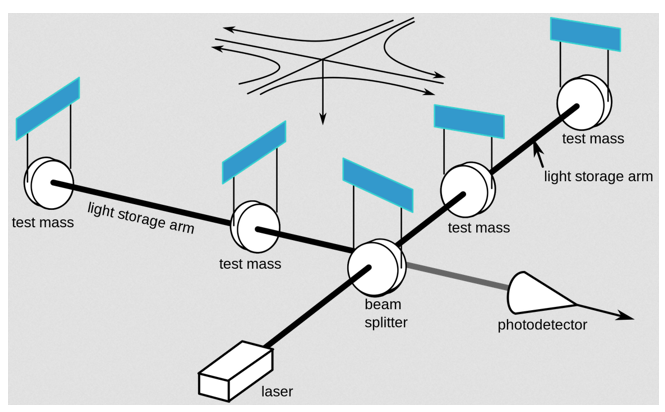
\includegraphics[width=1\textwidth]{figuras/interferometro.png}
\caption{Diagrama de um projeto básico de interferômetro. [Image: LIGO]}
\label{figinterferometer}
\end{figure}
 
Após a parada do LIGO nos periodos de 2010 à 2015 o observatorio foi parado para passar por um upgrade na capacidade de detecção e logo no inicio de suas atividade ele captou o primeiro sinal de uma colisão de buracos negros, há 1,3 bilhão de anos luz daqui, que levando ao prêmio Nobel de Física em 2017 \cite{abbott2016observation}. 
 
Quando um objeto denso e massivo é acelerado, ele cria ondas gravitacionais como as ondas que uma pedra lançada em um lago produz, e de acordo com Einstein, nada é mais denso e massivo do que um buraco negro. E o sistema binário, dois buracos negros giram um ao redor do outro, na primeira detecção que foi observada \cite{abbott2016observation}, um deles tinha a massa de 36 sóis e o outro de 29 conforme eles giram em órbita, emitem ondas gravitacionais e com isso perdem energia, conforme perdem energia, se aproximam ainda mais e giram ainda mais rápido quanto mais se aproximam, mais energia perdem e mais ondas emitem e mais se aproximam cada vez mais rápido até colidirem.

No final da explosão o buraco resultante ficou com 62 massas solares, os 3 sóis de diferença foram convertidos em ondas gravitacionais, conforme os buracos negros se aceleram antes da colisão, as ondas que emitem ficam cada vez mais intensas e cada vez mais frequentes, até virarem um gorjeio, que marca a colisão, um gorjeio emitido há mais de 1 bilhão de anos, uma explosão tão forte, que chacoalhou o espaço e o tempo e conseguimos captar daqui.

Agora temos a confirmação de que as ondas gravitacionais previstas há 100 anos existem, e sabemos como detectá-las. Em pouco tempo teremos detectores como LIGO em órbita da terra, com sensores há milhares de quilômetros de distância, capazes de detectar ondas gravitacionais ainda menores. Agora podemos captar as ondas emitidas pela explosão de supernovas ou pela fusão de estrelas de nêutrons formando buracos negros.


\section{Delimitação do Tema}

A natureza nem sempre pode ser observada em sua plenitude, mas sempre poderá ser simulada computacionalmente desde que existam os apropriados modelos computacionais. Neste sentido, a computação científica e numérica desempenha o papel de ferramenta fundamental da área da ciência da computação para o entendimento da natureza, explicitando fenômenos e dinâmicas muitas vezes não possíveis de serem observados pela limitada capacidade humana de observação.

Em particular, para a geração de modelos computacionais que venham a descrever a gravidade é necessário entender como o universo funciona. A teoria da Relatividade de Einstein \cite{albert1920realtivity} mostra que o espaço e o tempo não são entidades separadas. Desta forma, o espaço e o tempo formam um contínuum conhecido como espaço-tempo que participa da dinâmica dos eventos. As equações da Relatividade Geral de Einstein mostram que a dinâmica da matéria está conectada à curvatura do espaço-tempo. A gravidade é, portanto, uma manifestação da curvatura do espaço-tempo.

Um dos aspectos da dinâmica do espaço-tempo é radiação gravitacional. Prevista pela Teoria da Relatividade Geral em 1916, a descoberta das ondas gravitacionais tem sido um objetivo perseguido por cerca de 100 anos. A descoberta das ondas gravitacionais seria mais uma confirmação da Teoria da Relatividade Geral que se somaria às outras confirmações das Teoria de Einstein, tais como a deflexão da luz ao passar com objetos massivos como estrelas, lentes gravitacionais, a explicação do desvio do periélio do planeta Mercúrio, efeitos relativísticos nas órbirtas dos planetas, buracos negros, etc. 

Os efeitos Relativísticos de natureza gravitacionais são de grande importância à atual tecnologia e com aplicação à vida diária das pessoas. Um dos principais resultados da Teoria da Relatividade Geral foi a possibilidade de permitir a localização de coordenadas na superfície de planetas com extrema precisão (o equivalente ao georreferenciamento, contudo extraterrestre, a partir da Terra). A localização de coordenadas na superfície de planetas é uma das aplicações tecnológicas que só foi possível com uso da Teoria da Relatividade Geral. O resultado de tal tecnologia aplicado ao caso do planeta Terra foi o desenvolvimento da tecnologia do Sistema de Posicionamento Global GPS (Global Positioning System).

Por outro lado, a busca da detecção de ondas gravitacionais continua intensa, a análise e o tratamento computacional destas informações encontram-se na crisa da onda da tecnologia computacional para o entendimento de tal processo.

\section{Problema de Pesquisa}
Para que seja possível a detecção de GW é necessário um grande esforço contínuo dos detectores de GW e das instalações astronômicas e a natureza sensível a tempo dessas análises requer algoritmos que podem detectar e caracterizar eventos GW em tempo real e o custo computacional das buscas de filtros combinados aumenta significativamente quando se direciona as fontes de GW que abrangem um espaço de parâmetro dimensional mais alto.

A filtragem combinada, o algoritmo de detecção de GW mais sensível usado pelo LIGO, atualmente tem como alvo fontes binárias compactas com componentes alinhados à rotação em órbitas quase circulares.  Estudos recentes também indicam que essas buscas podem perder GWs geradas por populações binárias compactas formadas em ambientes estelares densos. Estender essas buscas com correspondência de modelos para direcionar BBHs de precessão por rotação, quase-circulares ou excêntricas é proibitivamente computacional \cite{george2018deep}.

Acelerar os algoritmos de estimação de parâmetros bayesianos offline, que normalmente duram de várias horas a alguns dias, não é uma tarefa trivial. a resposta para esses desafios tem sido o esforço continuo para reduzir o tamanho dos bancos de modelos usados para pesquisas GW baseadas em filtragem combinada \cite{indik2017reducing}. Com base nessas considerações, e percebendo que, para maximizar a ciência que se pode extrair das observações de GW, é essencial cobrir rapidamente um espaço de parâmetro mais profundo de fontes de motivação astrofísica, a comunidade da GW vem explorando instalações de computação de alto desempenho (HPC) de última geração para aumentar o conjunto de recursos computacionais para realizar a análise de dados GW em larga escala \cite{huerta2017boss,weitzel2017data}.


\section{Objetivos}
A seguir serão apresentados os objetivos geral (OG) e específicos (OE) que nortearão a condução desta pesquisa.

\subsection{Objetivo Geral}
A presente pesquisa tem como objetivo geral o desenvolvimento de procedimentos computacionais baseados em computação científica e numérica para o entendimento da dinâmica gravitacional do universo, contribuindo para uma nova área de pesquisa computacional designada de Astroinformatics com o desenvolvimento de bibliotecas computacionais para análise estatística dos resultados experimentais reais de medida das ondas gravitacionais. Para atingir esse objetivo geral foram propostos os objetivos específicos a seguir relacionados.
\subsection{Objetivos Específicos}
Para atingir o objetivo geral foram definidos os seguintes objetivos específicos: 
\begin{itemize}

\item Estudo introdutório dos processos de modelagem matemática para a geração das equações que governam as ondas gravitacionais;
\item Estudo das metodologias computacionais para a resolução de sistemas de equações diferenciais parciais acopladas;
\item E Desenvolvimento e implementação de bibliotecas numéricas para a solução de sistemas de equações diferenciais parciais em uma plataforma de GP/GPU (CUDA);
\item Simulações computacionais de ondas gravitacionais em uma plataforma baseada em GP/CPU (CUDA);
\item Estudo de inferência estatística e análise de ruídos para verificação de aderência entre os resultados obtidos pelo LIGO e as soluções numéricas obtidas.

\end{itemize}
\section{Justificativa}

Com base em todas as considerações descritas, precisamos de um novo paradigma para superar as limitações e os desafios computacionais dos algoritmos de detecção de GW existentes. Um candidato ideal seria a inteligencia artificial, mais especificamente as Machine Learning, a qual hoje é tendencia no mercado, que é uma área  altamente escalável que pode aprender diretamente a partir de dados brutos, sem qualquer recurso manual de engenharia, usando camadas hierárquicas profundas de “neurônios artificiais”. redes, em combinação com técnicas de otimização baseadas em retro-propagação e gradiente descendente \cite{barca2005treinamento}. A Machine Learning, especialmente com o auxílio da computação GPU, alcançou recentemente um imenso sucesso em aplicações comerciais e em inteligência artificial \cite{esteva2017dermatologist}, \cite{moravvcik2017deepstack}, \cite{van2016wavenet}, \cite{10.1007/978-3-319-44188-7_16}, e também tem sido aplicado em astrofísica \cite{george2017glitch}, \cite{george2017deepA}.
\chapter{Fundamentação Teórica}
\section{Ondas Gravitacionais}
\subsection{Introdução}

Qualquer objeto com massa exerce uma força de atração sobre outros objetos com massa, conhecida como “gravidade”. De acordo com a teoria da gravidade de Sir Isaac Newton \cite{newton1687philosophiae}, quaisquer dois objetos exercem uma atração gravitacional um sobre o outro de igual valor e sentido oposto, quando uma massa muda de posição, todo o campo gravitacional em todo o universo muda instantaneamente, e as forças gravitacionais resultantes são instantaneamente alteradas de acordo.

Mas a Teoria da Relatividade Geral de Einstein \cite{albert1920realtivity}, afirma que nenhuma informação pode viajar mais rápido que a velocidade da luz, incluindo informações sobre as posições de massa no universo, que são comunicadas através do campo gravitacional. A Relatividade Geral prevê que uma mudança no campo gravitacional viajará pelo universo à velocidade da luz e são exatamente essas mudanças no campo gravitacional que são as ondas gravitacionais.

De forma geral, as ondas gravitacionais podem ser pensadas como as ondas criadas quando jogamos pedras na superfície de um lago. Essas ondas são perturbações na geometria do próprio espaço-tempo emitidas por colisões violentas que acontecem no universo, que se propagam à velocidade da luz, carregando informações sobre suas origens, bem como pistas sobre a natureza da própria gravidade \cite{LSC-VIRGO, abbott2016observation, ramos2018teoria}.

\begin{figure}[ht]
\centering
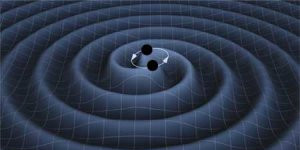
\includegraphics[width=.9\textwidth]{figuras/binary-wave_tn.jpg}
\caption{A impressão artística de ondas gravitacionais de dois buracos negros em órbita. [Imagem: T. Carnahan (NASA GSFC)]}
\label{fig:space-time}
\end{figure}

Ondas gravitacionais são criadas por massas móveis, da mesma forma que ondas eletromagnéticas são criadas por cargas em movimento. Mas como a gravidade é a mais fraca das quatro forças fundamentais (sendo as outras o eletromagnético, o nuclear fraco e o nuclear forte), as ondas gravitacionais são extremamente pequenas, produzindo um deslocamentos da ordem de \(10^{-18}\) metros, isto é, 1000 vezes menor que o diâmetro de um próton \cite{abbott2016observation}. Ondas dessa força serão produzidas por sistemas muito massivos que passam por grandes acelerações, como dois buracos negros em órbita que estão prestes a se fundir um com o outro. Como sistemas como esses são raros, essas fontes estarão a anos-luz de distância.

\subsection{Fontes e tipos de ondas gravitacionais}

Em geral, qualquer aceleração que não seja esfericamente ou cilindricamente simétrica produzirá uma onda gravitacional \cite{abbott2017gw170814}. Considere uma estrela que vai se transformar em uma supernova, esta explosão produzirá ondas gravitacionais se a massa não for ejetada de maneira esférica simétrica, embora o centro de massa possa estar na mesma posição antes e depois da explosão. Outro exemplo é uma estrela em movimento. Uma estrela perfeitamente esférica não produzirá uma onda gravitacional, mas sim uma estrela irregular \cite{abbott2017gw170817}.

Com base nessas diferentes fontes, os cientistas do LIGO definiram quatro categorias de ondas gravitacionais: Ondas Gravitacionais Contínuas, Ondas Gravitacionais de Sistemas Binários, Ondas Gravitacionais Estocásticas e Ondas Gravitacionais de colapso gravitacional. Cada categoria gera um conjunto único de "impressões digitais" ou assinaturas vibracionais características que os interferômetros do LIGO podem detectar e que os pesquisadores podem procurar nos dados do LIGO \cite{Christensen_2018}.

Ondas gravitacionais contínuas são produzidas por sistemas que têm uma frequência razoavelmente constante e bem definida. Exemplos disso são sistemas de estrelas binárias ou de buracos negros orbitando um ao outro ou uma única estrela girando rapidamente em torno de seu eixo com uma grande inchaço ou outras imperfeições na sua forma esférica. Espera-se que estas fontes produzam ondas gravitacionais comparativamente fracas, uma vez que elas evoluem ao longo de períodos de tempo mais longos e são geralmente menos catastróficas do que as fontes que produzem ondas gravitacionais de sistemas binários ou de colapso gravitacional \cite{beheshtipour2020deep}, Figura~\ref{figondacontinua}.

\begin{figure}[ht]
\centering
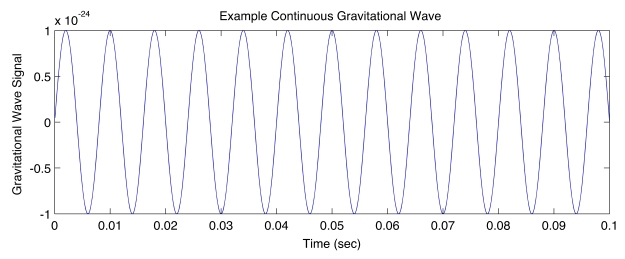
\includegraphics[width=.9\textwidth]{figuras/continuous_tn.jpg}
\caption{Um sinal de exemplo de uma fonte de onda gravitacional contínua. [Image: A. Stuver / LIGO]}
\label{figondacontinua}
\end{figure}

Ondas gravitacionais de sistemas binários são geradas durante o estágio final de vida de sistemas binários, onde os dois objetos se fundem em um. Esses sistemas são geralmente duas estrelas de nêutrons, dois buracos negros, ou uma estrela de nêutrons e um buraco negro cujas órbitas se degradaram até o ponto em que os dois objetos estão prestes a coalescer. À medida que os objetos giram em torno uma do outro, suas distâncias orbitais diminuem, retirando parte da energia orbital do sistema, enquanto suas velocidades aumentam \cite{Liu_2018}. Isso faz com que a frequência das ondas gravitacionais aumente até o momento da coalescência, Figura~\ref{figondainspiral}.

\begin{figure}[ht]
\centering
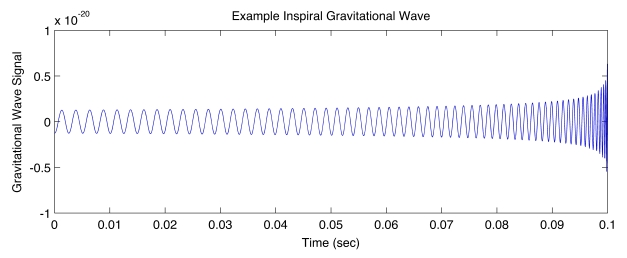
\includegraphics[width=.9\textwidth]{figuras/inspiral_tn.jpg}
\caption{Um sinal de exemplo de uma fonte de onda gravitacional de sistemas binários. [Image: A. Stuver / LIGO]}
\label{figondainspiral}
\end{figure}

As ondas gravitacionais de colapso gravitacional vêm de fontes desconhecidas ou imprevistas de curta duração. Há hipóteses de que alguns sistemas, como supernovas ou rajadas de raios gama, podem produzir ondas gravitacionais de colapso gravitacional, mas pouco se sabe sobre os detalhes desses sistemas para antecipar a forma que essas ondas terão \cite{Christensen_2018}, Figura~\ref{figondaruptura}.

\begin{figure}[ht]
\centering
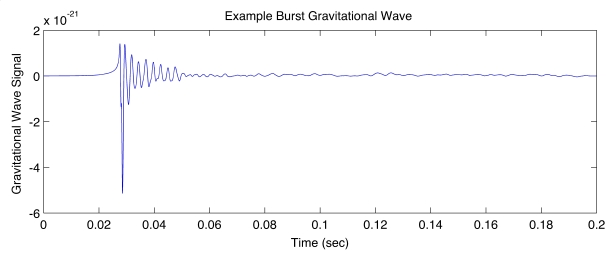
\includegraphics[width=.9\textwidth]{figuras/burst_tn.jpg}
\caption{Um sinal de exemplo de uma fonte de onda gravitacional de ruptura. [Image: A. Stuver / LIGO usando dados de C. Ott, D. Burrows e outros]}
\label{figondaruptura}
\end{figure}

Ondas gravitacionais estocásticas são as ondas gravitacionais relíquias da evolução inicial do universo. Assim como radiação cósmica de fundo em micro-ondas(Cosmic Micro-wave Background - CMB), que provavelmente é a luz residual do Big Bang, essas ondas gravitacionais surgem de um grande número de eventos aleatórios e independentes combinados para criar um fundo de ondas gravitacionais cósmicas. Essas pequenas ondas de todas as direções compõem o que é chamado de sinal estocástico, tendo um padrão aleatório que pode ser analisado estatisticamente, mas não previsto com precisão \cite{Christensen_2018}.

Espera-se que o Big Bang seja o principal candidato para a produção dos muitos processos aleatórios necessários para gerar ondas gravitacionais estocásticas e, portanto, podem conter informações sobre a origem e a história do universo \cite{Christensen_2018}, Figura \ref{figondaestocastica}.

\begin{figure}[ht]
\centering
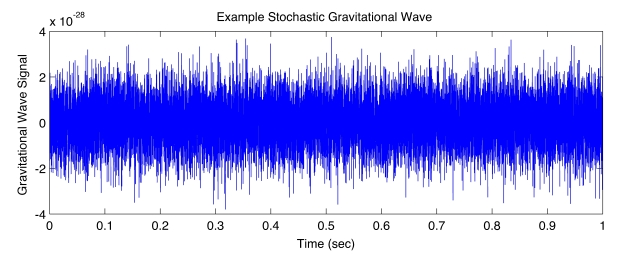
\includegraphics[width=.9\textwidth]{figuras/stochastic_tn.jpg}
\caption{Um sinal de exemplo de uma fonte de onda gravitacional estocástica. [Imagem: A. Stuver / LIGO]}
\label{figondaestocastica}
\end{figure}

\subsection{Equações de ondas Gravitacionais}

Uma maneira de se entender esse fenômeno matematicamente é através do cálculo que produz esse tipo de evento. Segundo a RG de Einstein, esses efeitos gravitacionais são descritos através da métrica $G_{\mu \nu}(x)$, que traz consigo informação acerca da curvatura do espaço-tempo.

Mas a equação de Einstein constitui um conjunto de 10 equações diferenciais parciais não lineares, o que, torna esse cálculo exaustivo e complexo. Uma maneira atrativa de se pensar nas equações de onda gravitacional produzidas por um sistema binário é tratar cada componente do sistema como um partícula. Segundo \cite{rubbo2007hands}, podemos fazer isto com a seguinte equação:

\begin{equation} \label{eqGW1}
\begin{split}
h(t) = \mathcal{A}(t)\cos \Phi(t),
\end{split}
\end{equation}

Na Equação \ref{eqGW1}, o $h(t)$ é a forma de onda gravitacional produzida pelos componentes(partículas) do sistema, também conhecida como deformação da onda gravitacional, $\mathcal{A}(t)$ é a amplitude dependente do tempo e $\Phi (t)$ é a fase da onda gravitacional. Ainda, segundo \cite{rubbo2007hands}, a amplitude $\mathcal{A}(t)$ pode ser expressa em termos dos parâmetros que caracterizam o sistema,

\begin{equation} \label{eqGW2}
\begin{split}
\mathcal{A}(t) = \frac{2(G\mathcal{M})^{5/3}}{c^4 r} \left(\frac{\pi}{P_{gw}(t)}\right)^{2/3} ,
\end{split}
\end{equation}
onde $G$ é a constante gravitacional de Newton, $c$ é a velocidade da luz, $r$ é a distância da luminosidade ao sistema binário e $P_{gw}(t)$ é o período da onda gravitacional. O valor $M \equiv (M_1 M_2)^{3/5}(M_1+M_2)^{-1/5}$ é a massa do \textit{chirp}\footnote{A massa do \textit{chirp} determina como o sistema evolui e o sinal de onda gravitacional emitido varia em amplitude e frequência, e é derivada da relação entre a massa total do sistema e a sua massa reduzida.} e comumente é usada na física das ondas gravitacionais, como uma escala de massa natural.

A fase das ondas gravitacionais, $\Phi (t)$, é análoga à fase para outro fenômeno das ondas, onde representa a localização do ciclo da onda que está colidindo com o detector no tempo $t$ e acompanha a evolução da amplitude da onda em função do tempo. A fase possui unidades de radianos e está relacionada à frequência da onda gravitacional $f_{gw}$ ou alternativamente ao período $P_{gw} = {f_{gw}^{-1}}$ pela integral da equação \ref{eqGW3}, onde, $\Phi_0$ é o valor da fase inicial, $\Phi_0=\Phi(t=0)$.

\begin{equation} \label{eqGW3}
\begin{split}
\Phi(t) = \Phi_0 + 2\pi \int_0^t \! \frac{{dt}^{'}}{P_{gw}(t^{'})}.
\end{split}
\end{equation}

Seguindo o exemplo dado em \cite{rubbo2007hands}, em que, os valores típicos da equação de amplitude de onda dado na Equação \ref{eqGW2}, foram substituídos por valores de um sistema binário de estrela de nêutrons localizado no centro de nossa galáxia, o mesmo afirma que as ondas gravitacionais são extremamente fracas e a amplitude de $\mathcal{A}$ é adimensional, portanto, a radiação gravitacional se manifesta na matéria ao induzir uma tensão. 

Em outros termos, a Equação \ref{eqGW1} proporciona a mudança relativa na distância entre dois pontos no espaço-tempo em função do tempo, tornando possível medir a separação entre duas massas e verificar se essas massas estão gerando uma onda gravitacional.

Como no eletromagnetismo, as ondas gravitacionais têm dois estados de polarização independentes designados por $\boldsymbol{+}$ e $\mathrm{X}$, como mostra a Figura \ref{figpolarization}. A polarização fornece, entre outras coisas, informação sobre a inclinação do plano orbital de um sistema binário em relação ao observador. Para um sistema binário, os dois estados são relacionados por uma mudança de fase de $90°$. Quando a linha de observação é paralela ao plano orbital do sistema, cada uma das componentes aparenta mover-se numa linha reta e neste caso possível, mostrar que a polarização das ondas gravitacionais emitidas será linear. 

\begin{figure}[ht]
\centering
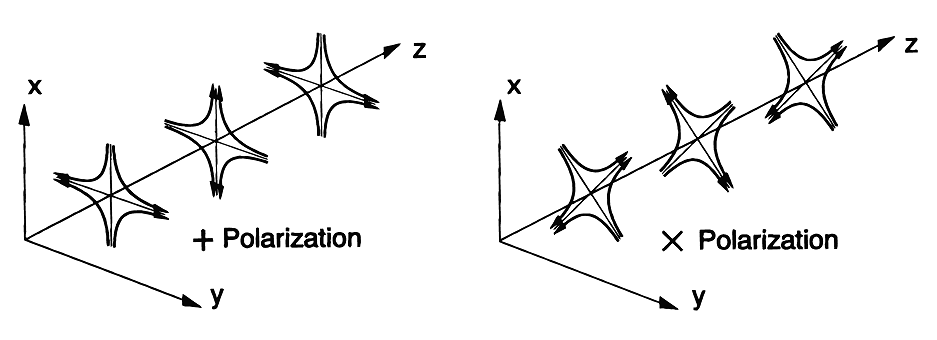
\includegraphics[width=.9\textwidth]{figuras/polarization.png}
\caption{Modos de polarização das ondas gravitacionais $\mathrm{h_{+}}$ e $\mathrm{h_{x}}$ propagando-se na direção $\mathrm{z}$. [Imagem: \cite{centrella2010black}]}
\label{figpolarization}
\end{figure}

Se, pelo contrário, a linha de observação for normal ao plano orbital, o movimento dos componentes será circular e a polarização observada será também circular. Entre estes dois casos limite existe uma gama de valores possível para a inclinação do plano orbital que pode em princípio ser deduzida através da polarização do sinal observado.

Consequentemente, a Equação \ref{eqGW1} captura a forma funcional dos dois estados de polarização. \cite{rubbo2007hands} afirma que ondas gravitacionais transportam energia e momento angular para longe do sistema binário, fazendo com que o período orbital diminua com o tempo, de acordo com

\begin{equation} \label{eqGW4}
\begin{split}
P_{orb}(t) = \left(P_0^{8/3} - \frac{8}{3}kt \right)^{3/8}
\end{split}
\end{equation}
onde $P_0$ é o período orbital no tempo $t = 0$, e $k$ é uma constante de evolução dada por:

\begin{equation} \label{eqGW5}
\begin{split}
k \equiv \frac{96}{5}(2\pi)^{8/3} \left(\frac{G\mathcal{M}}{c^3}\right)^{5/3}
\end{split}
\end{equation}

Como resultado do período orbital decrescente, os dois componentes binários se aproximaram lentamente, até o ponto em que colidem e coalesce em um único objeto remanescente, que ocorre quando $P_{orb}(t) = 0$.

Portanto, com a Equação \ref{eqGW1} é possível criarmos formas de ondas gravitacionais como mostra a Figura \ref{figmetade}. No entanto, é possível notar que a Equação \ref{eqGW1} não produz forma de onda, em que, o tempo é negativo, $P_{orb}(t) < 0$. Sendo assim, as formas de onda geradas por esse modelo não geram onda após a coalescência dos componentes. Devido a esta limitação este método de geração de ondas gravitacionais não será usado nesta pesquisa.

\begin{figure}[ht]
\centering
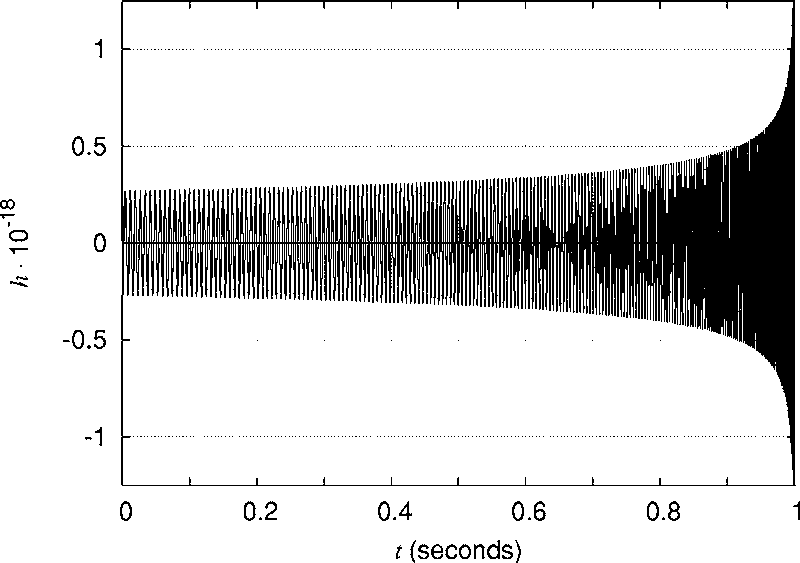
\includegraphics[width=.9\textwidth]{figuras/metade.png}
\caption{A forma de onda no último segundo antes da coalescência. Com a amplitude e a frequência do sinal aumentando com o tempo [Imagem: \cite{rubbo2007hands}]}
\label{figmetade}
\end{figure}

Esta é uma das maneiras que os astrônomos de ondas gravitacionais tem de extrair informações astrofísicas das formas de onda de sistemas binários observados. Claro que a análise de sinais reais é mais complexa. O principal desafio para a análise de dados reais é identificar o sinal oculto em um fluxo de dados com ruído. A abordagem mais comumente utilizada para esse problema na astronomia de ondas gravitacionais é usar a filtragem por coincidência. Se um sinal estiver presente em um fluxo de dados barulhento, o modelo fornecerá uma maneira de subtrair o ruído e deixar uma forma de onda limpa. Esta atividade assume que um modelo de sinal foi selecionado. Os astrônomos estimam os valores dos parâmetros astrofísicos que descrevem uma fonte de ondas gravitacionais a partir de formas de onda limpas \cite{rubbo2007hands}. 







\section{Redes Neurais Artificiais}

\subsection{Introdução às Redes Neurais Artificiais}

Qualquer que seja o organismo multicelular, independente da sua complexidade e organização, possui algum tipo de sistema nervoso que é responsável por alimentar o organismo através de entradas sensoriais sobre informações do ambiente em que o organismo vive. As informações coletadas são processadas e comparadas com experiências passadas e posteriormente são transformadas em ações apropriadas para a situação ou absorvidas em forma de conhecimento \cite{haykin1994neural}.

Para o organismo complexo, humano, o neurônio biológico é basicamente o dispositivo computacional elementar do sistema nervoso que possui muitas entradas e uma saída. As entradas ocorrem através das conexões sinápticas, que conectam a árvore dendrítica aos axônios de outras células nervosas. Os sinais que chegam por estes axônios são pulsos elétricos conhecidos como impulsos nervosos ou potenciais de ação, constituindo a informação que o neurônio processará de alguma forma para produzir como saída um impulso nervoso no seu axônio \cite{kovacs1996redes}. 

O cérebro humano possui uma capacidade incrível de absorção de conhecimento e é considerado o processador mais fascinante que existente, podendo desempenhar funções como percepção, intuição, inferência, reconhecimento de padrões, controle motor, entre outros. Ele possui cerca de $10^{11}$ de neurônios e cada neurônio pode receber de 1.000 a 10.000 contatos sinápticos em seu corpo e dendritos, que são responsáveis por todas as funções e movimentos do nosso organismo. Os neurônios estão conectados uns aos outros através de sinapses, e juntos formam uma grande rede, denominada Rede Neural, que proporciona uma fabulosa capacidade de processamento e armazenamento de informação \cite{kovacs1996redes}, Figura~\ref{figneuronios}. 

\begin{figure}[ht]
\centering
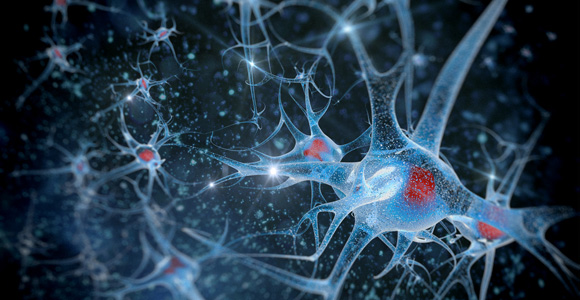
\includegraphics[width=1\textwidth]{figuras/axons.jpg}
\caption{Rede neural humana: o melhor processador de informações existente. [Imagem: \href{ https://neurogestion.wordpress.com}{ https://neurogestion.wordpress.com}]}
\label{figneuronios}
\end{figure}

\subsection{Redes Neurais Artificiais}

Há algumas décadas, surgiu a ideia de modelar, computacionalmente, as conexões neurais do cérebro humano, buscando reproduzir as características do neurônio biológico. Neste contexto, as redes neurais artificiais foram desenvolvidas, tomando-se como base as redes de neurônios cerebrais e sinapses biológicas do cérebro humano.

Uma rede neural é um sistema paralelo, distribuído, constituído pela interconexão de unidades básicas de processamento, denominadas neurônios artificiais, que têm a propensão natural para armazenar conhecimento experimental e torná-lo disponível para uso \cite{haykin2011neural}. Todo conhecimento adquirido pela rede se da através de um algoritmo de aprendizagem, cuja função é modificar os pesos de conexões entre os neurônios da rede, conhecidos como pesos sinápticos, de forma ordenada a fim de alcançar o mapeamento desejado.

\subsection{Neurônio Artificial}

A menor unidade básica de processamento de uma rede neural artificial é o neurônio, que recebe um sinal de entrada e produz um sinal de saída. O modelo de neurônio mais simples, comumente usado, e que engloba as principais características de uma rede neural biológica, paralelismo e alta conectividade, é o perceptron, representado na Figura~\ref{figperceptron}, que é composto por: m entradas (\(x_1, \ldots ,x_m\)), m pesos sinápticos (\(w_1, \ldots , w_m\)), uma variável de deslocamento linear \(b\) (do inglês: bias) e uma saída \(y\), descrito por:

\begin{equation} \label{eqRNA6}
\begin{split}
y = \theta(\sum_{i=1}^{m} x_i w_i + b)
\end{split}
\end{equation}

\begin{figure}[ht]
\centering
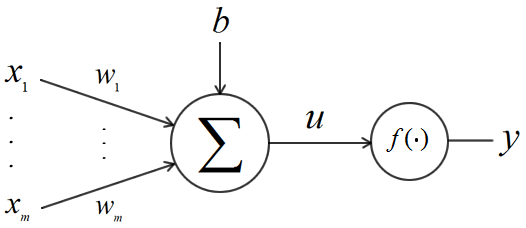
\includegraphics[width=.5\textwidth]{figuras/perceptron.png}
\caption{Modelo do neurônio artificial perceptron. [Imagem: \href{ http://computacaointeligente.com.br}{ http://computacaointeligente.com.br}]}
\label{figperceptron}
\end{figure}

A função \(\theta\) é conhecida como função de ativação ou função de transferência. Dentre as funções de ativação mais utilizadas estão a sigmoide e a tangente hiperbólica, definidas pelas equações abaixo, respectivamente \cite{articlefunclogtan}:

\begin{equation} \label{eq2}
\begin{split}
\theta(u) & = \frac{1}{1+ e^{-au}}\\
\theta(u) & = \frac{e^u - e^{-u}}{e^u + e^{-u}}
\end{split}
\end{equation}

\subsection{Arquitetura de uma RNA}

A arquitetura de uma RNA está relacionada com a maneira pela qual os seus neurônios estão organizados. De acordo com \cite{furtado2019redes}, as arquiteturas das RNAs são subdivididas em 3 classes: Rede Neural Feedforward de 1 camada, Rede Neural Feedforward Multicamadas e Redes Recorrentes ou Realimentadas. Além disso, a rede também é dividida em três tipos de camadas: a de entrada, a escondida e a de saída. 


As camadas podem ser classificadas em camadas de entrada, onde os padrões são apresentados à rede; camadas ocultas, onde é feita a maior parte do processamento; e a camada de saída, onde a conclusão do processamento é apresentada \cite{furtado2019redes}. Normalmente uma rede neural possui uma camada de entrada, uma camada de saída e \(k\) camadas ocultas, no qual \(k\) é definido empiricamente e varia de acordo com o problema.

Redes neurais do tipo Feedforward são redes de múltiplas camadas, ou seja, elas tem \(k\) camadas ocultas, no qual, a informação propaga-se da entrada para a saída, no caso, os sinais provenientes dos neurônios de uma camada só podem estimular os neurônios da camada seguinte. Quando a rede possuir todos os nós de uma camada comunicando-se com todos os nós da camada posterior, ela é dita totalmente conectada. Caso alguma das conexões sinápticas não esteja ligada com a camada subsequente, a rede é dita parcialmente conectada \cite{furtado2019redes}. A Figura \ref{figredeFeedforwardMulticamada} representa uma rede Feedforward multicamada de uma camada oculta totalmente conectada, ou seja, $k=1$.

% \begin{figure}[h]
% \centering
% 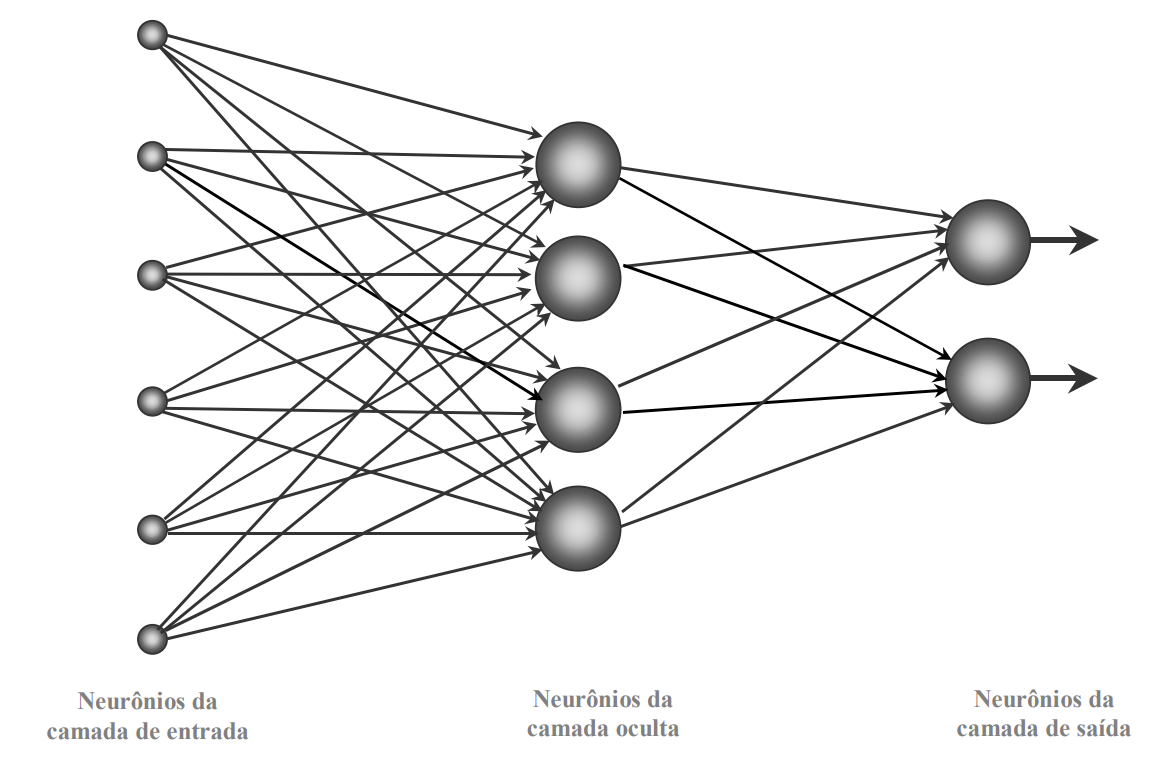
\includegraphics[width=.75\textwidth]{figuras/multicamadas.png}
% \caption{Exemplo de rede neural artificial do tipo Feedforward multicamadas. [Imagem: \cite{furtado2019redes}]}
% \label{figredeFeedforwardMulticamada}
% \end{figure}

\begin{figure}[h]
\centering
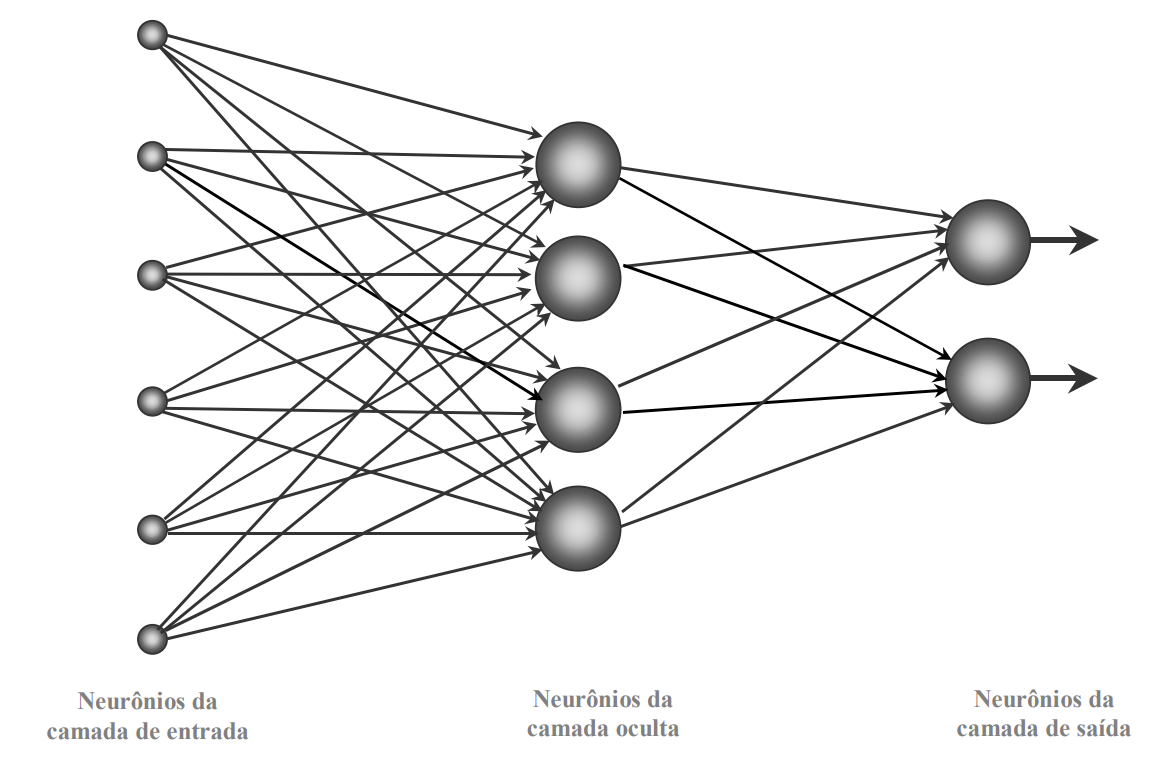
\includegraphics[width=.75\textwidth]{figuras/multicamadas.png}
\caption{Exemplo de rede neural artificial do tipo Feedforward multicamadas. [Imagem: \cite{furtado2019redes}]}
\label{figredeFeedforwardMulticamada}
\end{figure}

\subsection{Algoritmo de Treinamento}

A arquitetura da rede define, dentre outros parâmetros, a que tipo de treinamento a rede será submetida, capacitando-a a resolver o problema. No processo de treinamento a rede ‘aprende’ através de exemplos que relacionam as entradas e saídas do problema a ser solucionado. Essa abordagem é conhecida como aprendizado supervisionado. Dentre os algoritmos conhecidos, para solucionar esse tipo de problema, o mais utilizado é o backpropagation \cite{rumelhart1986learning}. A ideia do algoritmo é estimar os valores dos pesos e bias minimizando o erro entre a entrada e a saída desejada. O erro \(E\) cometido pela rede é calculado por:

\begin{equation} \label{eq3}
\begin{split}
E = \frac{1}{2} \sum_{i=1}^{p} \sum_{j=1}^{n} (d_{j}^{i} - y_{j}^{i})^2
\end{split}
\end{equation}
no qual, \(p\) é o número exemplos a ser utilizados no treinamento, n é o número de saídas da rede e, finalmente, \(d\) e \(y\) são as saídas desejadas e obtidas, respectivamente, para a entrada em questão.

Se o erro \(E\) encontrado for retropropagado (termo que foi derivado do nome do algoritmo backpropagation) pela rede, isto é, se o erro for propagado a partir da camada de saída até a camada de entrada, ela tentará estabelecer o quanto cada sinapse contribuiu para o erro, e este será usado para ajustá-las. A regra de atualização de cada peso sináptico da rede é calculado pela seguinte equação:

\begin{equation} \label{eqRNA4}
\begin{split}
W = W + \Delta W \therefore \Delta W = - \alpha\frac{\partial E}{\partial W}
\end{split}
\end{equation}

onde, \(\alpha\) é conhecido como taxa de aprendizado, que, resumidamente, indica o ‘tamanho do passo’ do gradiente rumo a minimização. O sinal negativo indica a busca por uma alteração no peso que reduza \(E\), sendo assim, quanto menor o erro, melhor a rede estará mapeando o problema.


% \subsection{Introdução às Redes Neurais Artificiais}

% A simulação cognitiva é uma técnica que permite imitar a forma e o comportamento de um organismo realizando suas atividades, estando inspirada em conceitos desenvolvidos na modelagem cognitiva, e utiliza os formalismos de representação de estruturas de domínio da Inteligência Artificial, que é um vasto campo que contém diversos componentes importantes, como as Redes Neurais Artificiais (RNAs) \cite{furtado2019redes}.

% Uma rede neural artificial (RNA) é basicamente um modelo computacional inspirado biologicamente. Ele tenta simular o processo de informação de um cérebro \cite{franchini2018artificial, yalccinreconfigurable}. Ele consiste em uma estrutura conexionista, na qual o processamento é distribuído por um elevado número de elementos processadores, os neurônios, amplamente interligados através de conexões com um determinado valor que estabelece o grau de conectividade entre estes, denominado peso da conexão ou sinapse e emula as propriedades decorrentes do alto grau de paralelismo e conectividade dos sistemas biológicos \cite{furtado2019redes}.

% Existem muitos tipos de RNA, mas, em geral, uma RNA é matematicamente um aproximador de função universal \cite{Cybenko1989}. Portanto, problemas com um alto número de observações e sem um modelo de análise conhecido são excelentes candidatos a sistemas baseados em soluções de RNA. Os recursos de generalização de informações e aprendizado da RNA são a base para gerar soluções para uma grande classe de problemas, como classificação, reconhecimento, clustering, previsão, regressão, mineração de dados, entre outros.

% \subsection{Histórico das Redes Neurais Artificiais}

% A primeira pesquisa relacionada ao desenvolvimento de um neurônio artificial biológico teve início na década de 40 do século passado, as primeiras informações sobre a neuro computação datam de 1943, em artigos de McCulloch e Pitts \cite{mcculloch1943logical}, que desenvolveram um modelo matemático de neurônio biológico artificial e sugeriam a construção de uma máquina baseada ou inspirada no cérebro humano, porém essa ideia não conseguiu desempenhar a tarefa de aprendizado.

% Desde então, pesquisadores começaram a desenvolver estudos relacionados com a forma de aprendizagem das redes biológicas e artificiais devido à experiência adquirida e sobre sua capacidade de executar determinadas funções (BRAGA et al., 2000).

% Em 1949 Donald Hebb escreveu um livro intitulado “A Organização do Comportamento” \cite{hebb1949organization}, onde apresentou uma hipótese a respeito da maneira com que a força das sinapses no cérebro se altera em resposta à experiência. Ele sugeriu que as conexões entre neurônios que são ativadas ao mesmo tempo tendem a se fortalecer, enquanto que as outras conexões tendem a se enfraquecer. Essa ideia fez dele o primeiro a propor uma lei de aprendizagem específica para as sinapses dos neurônios e esta hipótese passou a influenciar decisivamente na evolução da teoria de aprendizagem em RNAs, inspirando muitos outros pesquisadores a perseguirem a mesma ideia.

% Em 1951 foi construído primeiro neuro computador, denominado Calculadora Estocástica Neural-Analógica de Reforço (Stochastic Neural Analog Reinforcement Calculator - SNARC), por Mavin Minsky \cite{minsky1952neural}. Porem o SNARC nunca executou qualquer função de processamento de informação interessante. Somente mais tarde, em 1957 e 1958, que houve o primeiro desenvolvimento bem-sucedido de um neuro computador (Mark I Perceptron). Ele foi criado por Frank Rosenblatt, Charles Wightman e outros. Rosenblatt introduziu uma nova abordagem para o problema de reconhecimento de padrões com o desenvolvimento do Perceptron e também propôs um algoritmo para o ajuste dos pesos \cite{rosenblatt1958perceptron}.

% Por volta do mesmo período, Bernard Widrow, com a ajuda de alguns estudantes, desenvolveu um novo tipo de elemento de processamento de redes neurais chamado de Adaline (abreviação de Adaptive Linear Neuron ou posteriormente de Adaptive Linear Element) e mais tarde a sua generalização multidimensional, o Madaline (abreviação de Many ADALINE)\cite{widrow1960adaptive}. Esta rede era equipada com uma nova lei de aprendizado, conhecida como "Regra Delta", que depois foi generalizada para redes com modelos neurais mais elaborados, que diferente do Perceptron ainda permanece em uso \cite{furtado2019redes}.

% Os anos seguintes foram marcados por um entusiasmo exagerado criada pelos próprios pesquisadores desta área, que prometiam máquinas tão poderosas quanto o cérebro humano e que surgiriam em um curto espaço de tempo não acompanhada de resultados à altura, o que agravou a queda de financiamentos para as pesquisas e tirou a credibilidade dos estudos desta área \cite{furtado2019redes}.

% Em 1969, Minsky e Papert publicaram o livro “Perceptrons - An Introduction to Computational Geometry” \cite{minsky1969perceptrons}. Neste livro os autores explicam às limitações básicas das redes perceptrons, como por exemplo a impossibilidade de se implementar regras lógicas simples, como o ou-exclusivo. Neste livro os autores demonstraram que a rede perceptron, é capaz de executar as operações booleanas AND e OR, mas não é capaz de executar outras operações, como XOR (ou-exclusivo). Além do mais, os mesmos não acreditavam que uma arquitetura adequada em conjunto com um algoritmo de ajuste dos pesos pudesse ser desenvolvida de forma a superar este problema.

% Após a publicação deste livro as pesquisas na área de redes neurais paralisaram por um tempo. Os pesquisadores passaram a buscar por soluções em outras áreas, como da lógica matemática, que na época, encontrava-se em franca expansão, devido às grandes conquistas realizadas na área de computação \cite{nocaoderna}.

% Este período de pesquisa silenciosa perdurou até meados de 1982, com poucas publicações devido aos fatos ocorridos anteriormente. Entretanto, aqueles que pesquisavam nesta época como Teuvo Kohonen, Stephen Grossberg, B.Widrow, James Anderson, Edoardo Caianiello, Kunuhito Fukushima, Igor Aleksander e todos os que se seguiram no decorrer destes anos passaram a publicar diversas propostas para o desenvolvimento e para as aplicações de redes neurais, conseguindo assim, novamente estabelecer um campo concreto para o renascimento da área. O alto pode computacional, o desenvolvimento de novos algorítimos de aprendizado e o aprofundamento sobre a estrutura cerebral, foram os fatores que mais contribuíram para a retomada do interesse pela exploração das redes neurais artificiais \cite{nocaoderna}.

% Quando John Hopfield, renomado físico de reputação mundial e ganhador do Prêmio Nobel, se interessou pela neuro computação, ele incentivou e difundiu os princípios desta área entre importantes cientistas, matemáticos e tecnólogos altamente qualificados.

% Em 1986 o campo de pesquisa se extasiou com o desenvolvimento de um método para ajuste de parâmetros de redes não-recorrentes de múltiplas camadas. Este método, baseado em um algoritmo denominado retropropagação (backpropagation) \cite{rumelhart1986learning}, tornou-se largamente conhecido após a publicação do livro “Processamento Distribuído Paralelo” editado por David Rumelhart e James McClelland, fazendo com que pesquisadores das mais diferentes áreas passassem a visualizar interessantes aplicações para redes neurais artificiais.

% Desde então conferencias e institutos de pesquisa nesta área vem surgindo cada vez mais. E Recentemente, redes neurais artificiais tem se tornado a solução para muitas aplicações computacionais, tais como: reconhecimento de padrões, processamento de imagens, sistemas de controle, robótica, identificação de sistemas e astronomia.

% \subsection{Redes Neurais Biológicas}

% Qualquer que seja o organismo multicelular, independente da sua complexidade e organização, possui algum tipo de sistema nervoso que é responsável por alimentar o organismo através de entradas sensoriais sobre informações do ambiente em que o organismo vive. As informações coletadas são processadas e comparadas com experiências passadas e posteriormente são transformadas em ações apropriadas para a situação ou absorvidas em forma de conhecimento \cite{haykin1994neural}.

% Para o organismo complexo, humano, o neurônio biológico é basicamente o dispositivo computacional elementar do sistema nervoso que possui muitas entradas e uma saída. As entradas ocorrem através das conexões sinápticas, que conectam a árvore dendrítica aos axônios de outras células nervosas. Os sinais que chegam por estes axônios são pulsos elétricos conhecidos como impulsos nervosos ou potenciais de ação, constituindo a informação que o neurônio processará de alguma forma para produzir como saída um impulso nervoso no seu axônio \cite{kovacs1996redes}. 

% O cérebro humano possui uma capacidade incrível de absorção de conhecimento e é considerado o processador mais fascinante que existente, podendo desempenhar funções como percepção, intuição, inferência, reconhecimento de padrões, controle motor, entre outros. Ele possui cerca de $10^{11}$ de neurônios e cada neurônio pode receber de 1.000 a 10.000 contatos sinápticos em seu corpo e dendritos, que são responsáveis por todas as funções e movimentos do nosso organismo. Os neurônios estão conectados uns aos outros através de sinapses, e juntos formam uma grande rede, denominada Rede Neural, que proporciona uma fabulosa capacidade de processamento e armazenamento de informação \cite{kovacs1996redes}, Figura~\ref{figneuronios}. 

% \begin{figure}[ht]
% \centering
% 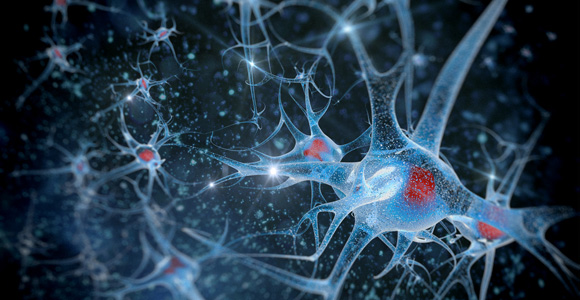
\includegraphics[width=1\textwidth]{figuras/axons.jpg}
% \caption{Rede neural humana: o melhor processador de informações existente. [Imagem: \href{ https://neurogestion.wordpress.com}{ https://neurogestion.wordpress.com}]}
% \label{figneuronios}
% \end{figure}

% O sistema nervoso é formado por um conjunto extremamente complexo de neurônios. Nesses, a comunicação é realizada através de impulsos. Quando um impulso é recebido, o neurônio o processa, e passado um limite de ação, dispara um segundo impulso que produz uma substância neurotransmissora o qual flui do corpo celular para o axônio que por sua vez pode estar ou não conectado a um dendrito de outra célula. O neurônio que transmite o pulso pode controlar a frequência de pulsos aumentando ou diminuindo a polaridade na membrana pós-sináptica. Eles têm um papel essencial na determinação do funcionamento, comportamento e do raciocínio do ser humano. 

% Ao contrário das redes neurais artificiais, redes neurais biológicas não transmitem sinais negativos, sua ativação é medida pela frequência (contínua e positiva) com que emite os pulsos. As redes neurais biológicas não são uniformes como as redes artificiais e apresentam uniformidade apenas em alguns pontos do organismo. Seus pulsos não são síncronos ou assíncronos, devido ao fato de não serem contínuos, o que as difere das redes artificiais. 

% Baseada na célula nervosa básica chamada neurônio, como qualquer célula biológica, o neurônio é delimitado por uma fina membrana celular que além da sua função biológica normal, possui propriedades que permitem a transmissão de sinais elétricos. A Figura \ref{figneuroniobiologico} ilustra a aparência de uma célula nervosa (neurônio) e de acordo  com  Braga  (2010,  p.  5),  em  uma  Rede  Neural  Biológica cada neurônio é dividido em três principais seções: o corpo do neurônio, os dendritos e o axônio.

% \begin{enumerate}[label={\alph*)}]
%     \item Dendritos: Tem por função, receber os estímulos transmitidos por outros neurônios;
%     \item Corpo do neurônio: Também chamado de soma, o qual é responsável por coletar e combinar informações vindas de outros neurônios. É o centro dos processos metabólicos da célula nervosa;
%     \item Axônio: Responsável pela condução do impulso nervoso na saída do neurônio.
% \end{enumerate}

% \begin{figure}[ht]
% \centering
% 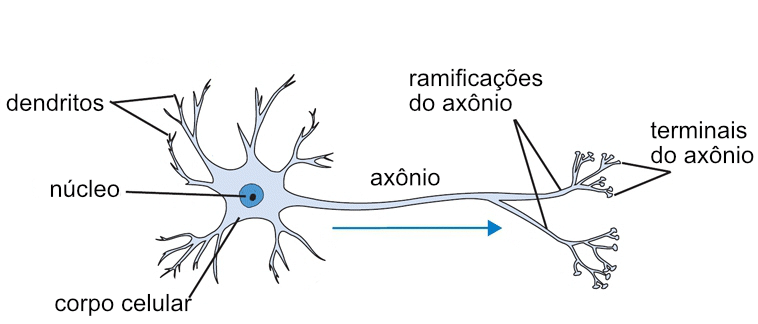
\includegraphics[width=1\textwidth]{figuras/neuronio.png}
% \caption{Representação de um neurônio biológico. [Imagem adapitada: \href{http://cs231n.github.io/neural-networks-1/}{http://cs231n.github.io/neural-networks-1/}]}
% \label{figneuroniobiologico}
% \end{figure}

% Na  Figura  \ref{figneuroniobiologico} é representado o neurônio biológico, onde os impulsos nervosos são receptados através dos dendritos que percorrem o núcleo envolvido pelo corpo do neurônio, passando pelo axônio até seus terminais para formarem as sinapses, que formam as interações entre os neurônios \cite{haykin2007redes}

% \subsection{Redes Neurais Artificiais}

% Há algumas décadas, surgiu a ideia de modelar, computacionalmente, as conexões neurais do cérebro humano, com intuito de emergir comportamentos inteligentes em máquinas. Neste contexto, surgiu as Redes Neurais Artificiais (RNA's), inspiradas na própria natureza das redes de neurônios cerebrais e sinapses biológicas.

% O trabalho em RNA's, comumente chamadas de “redes neurais” (RN), foi motivado desde o início pelo reconhecimento de que o cérebro humano computa de uma forma totalmente diferente do computador digital convencional. O cérebro é um computador altamente complexo, não linear e paralelo \cite{haykin2009neural}.

% Uma rede neural artificial é um sistema de processamento paralelo de informações constituído pela interconexão de unidades básicas de processamento, denominadas neurônios artificiais, que tem a propensão natural para armazenar conhecimento experimental e torná-lo disponível para o uso \cite{haykin2009neural}. Todo conhecimento adquirido pela rede se da através de um algoritmo de aprendizagem, cuja função é modificar os pesos de conexões entre os neurônios da rede, conhecidos como pesos sinápticos, de forma ordenada a fim de alcançar o mapeamento desejado.

% O neurônio artificial é a menor unidade de processamento de uma rede neural, que recebe sinais de entrada e produzem sinais de saída. O modelo de neurônio mais simples, e que engloba as principais características de uma rede neural biológica, paralelismo e alta conectividade, foi proposto por McCulloch e Pitts em 1943 \cite{mcculloch1943logical}

% O neurônio de McCullock e Pitts, apesar de simples, ainda é utilizado. Este modelo consistia basicamente em m terminais de entrada (dendritos) que recebem m valores \(x_1, \ldots ,x_m\) (que representam as ativações dos neurônios anteriores) e apenas um terminal de saída \(y\) (representando o axônio). As sinapses foram representadas por pesos (\(w_1, \ldots , w_m\)), acoplados nos terminais de entrada. Tais pesos podem possuir valores positivos ou negativos. Assim, o efeito da sinapse de um neurônio i pré-sináptico que emite um sinal \(x_i\) é \(w_{i}x_{i}\). O percentual de excitação de tal modelo é feito somando todas as sinapses correspondentes \(\sum w_{i}x_{i}\). 

% \begin{figure}[ht]
% \centering
% 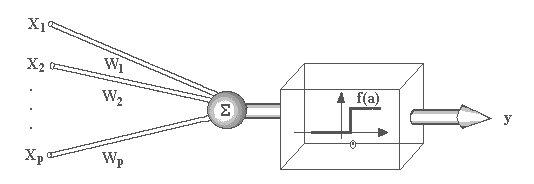
\includegraphics[width=1\textwidth]{figuras/Neuronio_McCulloch.png}
% \caption{Neurônio Artificial projetado por McCulloch e Pitts}
% \label{figneuronioMcCulloch}
% \end{figure}

% O disparo ou não do neurônio então se dá comparando o resultado dessa soma com o limiar de ativação, a partir de uma função de ativação. Por se tratar de um modelo binário, a saída do neurônio de McCulloch e Pitts pode ser pulso (1) ou não-pulso (0).

% Matematicamente o modelo apresentado na Figura \ref{figneuronioMcCulloch} pode ser representado por:

% \begin{equation} \label{eqRNA6}
% \begin{split}
% u_k = \sum_{j=1}^{m} w_{kj} x_i
% \\e
% \\ y_k = \theta(u_k)
% \end{split}
% \end{equation}

% A função de ativação, também conhecida como função restritiva, tem por objetivo limitar a amplitude do sinal de saída do neurônio. Para o modelo de McCulloch e Pitts, a função de ativação é a função de limiar, representada matematicamente como:

% \begin{equation} \label{eqRNA7}
% \begin{split}
% \theta(v) = \left\{ \begin{array}{rcl}1 & se & v\ge0
% \\ 0 & se & v<0
% \end{array}\right.
% \end{split}
% \end{equation}

% O modelo de McCulloch e Pitts pode ser esquematizado em uma forma mais geral de forma a possibilitar diversas aplicações: pode-se inserir um polarizador ou bias na entrada do neurônio e alterar a função de ativação \( \theta(·)\), utilizando para isso outras funções. O bias tem o efeito de aumentar ou diminuir a entrada líquida da função de ativação. Quatro elementos básicos podem ser identificados nesse modelo mais geral, a saber:

% \begin{enumerate}
%     \item Sinapses.
%     \item Somador.
%     \item Função de Ativação.
%     \item Bias (polarizador).
% \end{enumerate}

% O funcionamento do neurônio da Figura \ref{figneuronioMcCulloch}, acrescido do bias, pode ser descrito de forma matemática como:

% \begin{equation} \label{eqRNA8}
% \begin{split}
% y_k = \theta(u_k + b_k)
% \end{split}
% \end{equation}

% Este modelo se apresenta constante para quase todas as Redes Neurais, variando somente a função de ativação. Esta limita a amplitude do sinal de saída do neurônio. Normalmente a faixa de saída está em um intervalo fechado [0, 1] ou alternativamente em [-1, 1], podendo também este intervalo de saída estar entre (\(- \infty, + \infty\)) \cite{furtado2019redes}.

% \subsection{Funções de Ativação}

% Na equação \ref{eqRNA8}, a função de ativação processa o conjunto de entradas recebidas e o transforma em estado de ativação. Entre os diversos tipos de funções de ativação, as mais comuns estão representadas na Figura \ref{figfuncAtivação}. 

% \begin{figure}[ht]
% \centering
% 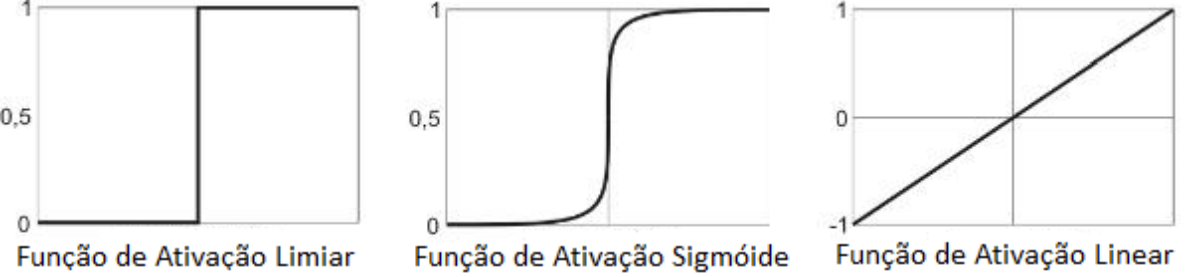
\includegraphics[width=1\textwidth]{figuras/funcAtivacao.png}
% \caption{Funções de ativação [Imagem adaptada: \cite{haykin1994neural}]}
% \label{figfuncAtivação}
% \end{figure}

% O tipo de função de ativação a ser utilizada é definido conforme a finalidade da construção da rede neural artificial. Permitir que a função de ativação assuma valores negativos pode trazer benefícios em alguns projetos e não trazer benefícios em outros.

% A função de ativação Limiar, utilizada no neurônio de McCulloch e Pitts, limita a saída do neurônio a apenas dois valores (binário: 0 e 1, ou bipolar: -1 e 1). Normalmente é utilizada em neurônios que tomam decisões binárias, como nos classificadores, definida como mostrado na equação \ref{eqRNA7}.

% A função de linear por partes e do tipo de função que pode ser visto como uma aproximação de um amplificador não linear, e possui a seguinte definição:

% \begin{equation} \label{eqRNA9}
% \begin{split}
% \theta(v) = \left\{ \begin{array}{rcl}1 & se & v\ge1/2
% \\ v & se & -1/2<v<+1/2
% \\ 0 & se & v<-1/2
% \end{array}\right.
% \end{split}
% \end{equation}

% Já a função Sigmoide é muito comum na construção de redes neurais artificiais e é utilizada por vários modelos de aplicações, apresenta um gráfico contínuo e suave, é monotônica e também diferenciável em qualquer ponto. A função Sigmoide pode ser representada pela função logística ou pela função tangente hiperbólica. Fundamentalmente, a diferença entre elas está nos intervalos nos quais são delimitadas. A função logística é definida pela equação \ref{eqRNA10}, onde o $b$ é o parâmetro de inclinação da função:

% \begin{equation} \label{eqRNA10}
% \begin{split}
% \theta(v) = \frac{1}{1+e^{-bv}}
% \end{split}
% \end{equation}

% Na função tangente hiperbólica, as funções de ativação definidas nas Equações \ref{eqRNA8}, \ref{eqRNA9} e \ref{eqRNA10} se estendem de $0$ a $+1$. Algumas vezes é desejável que a função de ativação se estenda de $-1$ a $+1$, assumindo neste caso uma forma anti-simétrica em relação à origem. Possui a seguinte definição:

% \begin{equation} \label{eqRNA11}
% \begin{split}
% \theta(v) = \tanh(v)
% \end{split}
% \end{equation}

% \subsection{Arquiteturas de Redes Neurais}

% % A maioria dos modelos de redes neurais possui alguma regra de treinamento, onde os pesos de suas conexões são ajustados de acordo com os padrões apresentados. Em outras palavras, elas aprendem através de exemplos (padrões).

% A arquitetura de uma rede neural está relacionada com a maneira pela qual os neurônios da mesma estão organizados. Em geral elas são subdivididas em 3 classes: Rede Neural Feedforward de 1 camada, Rede Neural Feedforward Multicamadas e Redes Recorrentes ou Realimentadas.

% A rede também é dividida em três tipos de camadas: a de entrada, a escondida e a de saída. As camadas de entrada e saída são intuitivas e representam o número de entradas e saídas do problema em questão. Já a escondida é a camada que fará a maior parte do processo de aprendizagem da rede. Normalmente uma rede neural possui uma camada de entrada, uma camada de saída e \(k\) camadas escondidas, no qual \(k\) é definido empiricamente e varia de acordo com o problema. 

% Redes neurais Feedforward (em português costumam traduzir como alimentação direta ou avante) apresenta uma organização similar à do córtex humano, em especial, a de 1 camada, em que, os neurônios se dispõem em camadas paralelas e consecutivas, e os axônios se estendem sempre no mesmo sentido, isto é, a informação propaga-se da entrada para a saída, não existindo portanto ligações entre os neurônios de uma mesma camada ou com camadas anteriores como pode ser visto na Figura \ref{figredeFeedforwardcamadaunica}, os nós da camada de entrada se comunicam diretamente com a camada de saída (nós computacionais). Suas principais aplicações são em memória associativa e no reconhecimento de padrões.

% \begin{figure}[ht]
% \centering
% 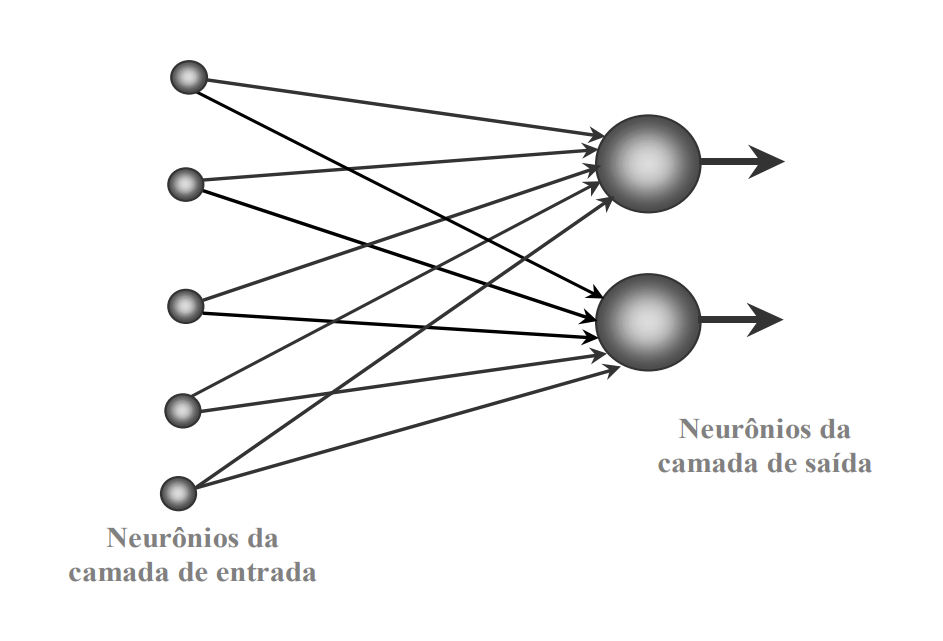
\includegraphics[width=.6\textwidth]{figuras/camada_unica.png}
% \caption{Exemplo de rede neural artificial do tipo Feedforward de 1 camada. [Imagem \cite{furtado2019redes}]}
% \label{figredeFeedforwardcamadaunica}
% \end{figure}

% Redes neurais do tipo Feedforward Multicamadas são redes de múltiplas camadas, ou seja, elas tem \(k\) camadas escondidas e seguem a mesma logica das redes de uma única camada, no caso, os sinais provenientes dos neurônios de uma camada só podem estimular os neurônios da camada seguinte, não existindo realimentação. Quando a rede possuir todos os nós de uma camada comunicando-se com todos os nós da camada posterior, ela é dita totalmente conectada. Caso alguma das conexões sinápticas não esteja ligada com a camada subsequente, a rede é dita parcialmente conectada. A Figura \ref{figredeFeedforwardMulticamada} representa uma rede Feedforward multicamada totalmente conectada. Suas principais aplicações são em reconhecimento de padrões, aproximador universal de funções e em controle.

% \begin{figure}[h]
% \centering
% 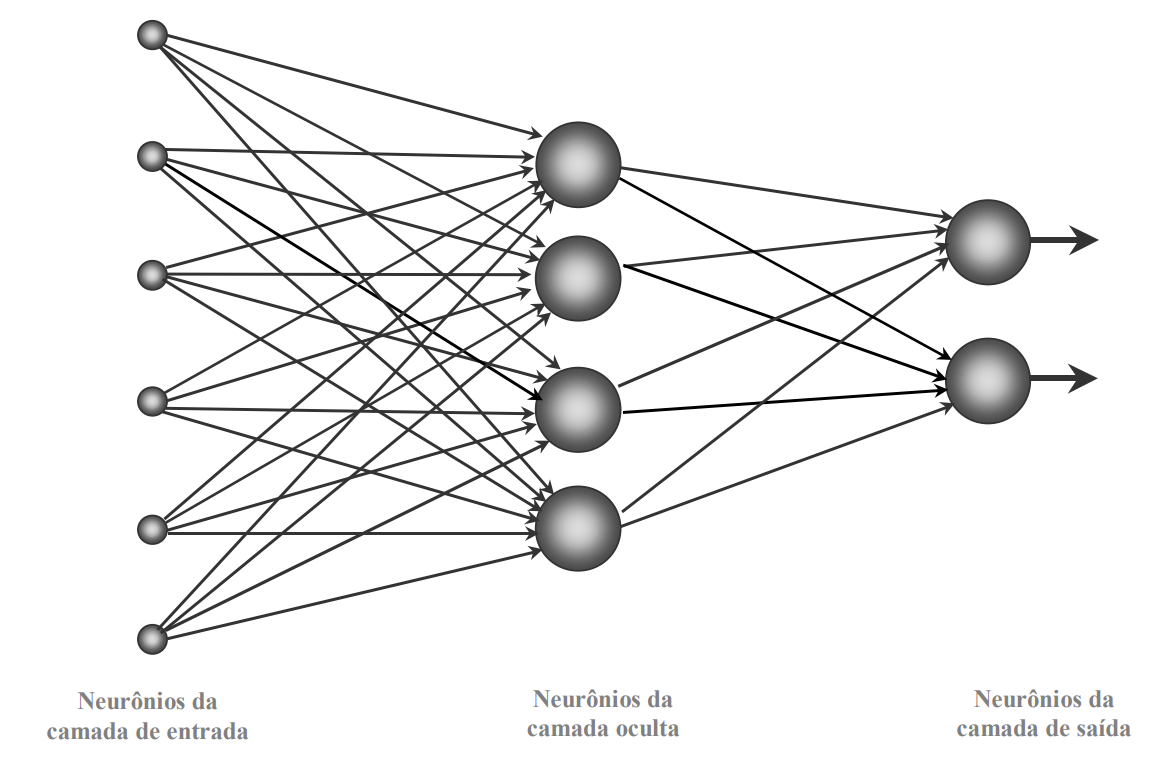
\includegraphics[width=.75\textwidth]{figuras/multicamadas.png}
% \caption{Exemplo de rede neural artificial do tipo Feedforward multicamadas. [Imagem: \cite{furtado2019redes}]}
% \label{figredeFeedforwardMulticamada}
% \end{figure}

% Redes Recorrentes ou Realimentadas distingue-se das redes neurais do tipo Feedforward por permitir a realimentação entre neurônios de camadas diferentes, ou ainda por fazer uma realimentação do neurônio com a sua própria saída (selffeedback). A Figura \ref{figredeRecorrente} apresenta uma rede recorrente com self-feedback e sem neurônios na camada intermediária. Suas principais aplicações são em sistemas dinâmicos, memória associativa, previsão e estimação, otimização e em controle, são mais poderosas que as outras, porém são bem mais complexas, tanto para utilização quanto para a análise dos resultados apresentados.

% \begin{figure}[ht]
% \centering
% 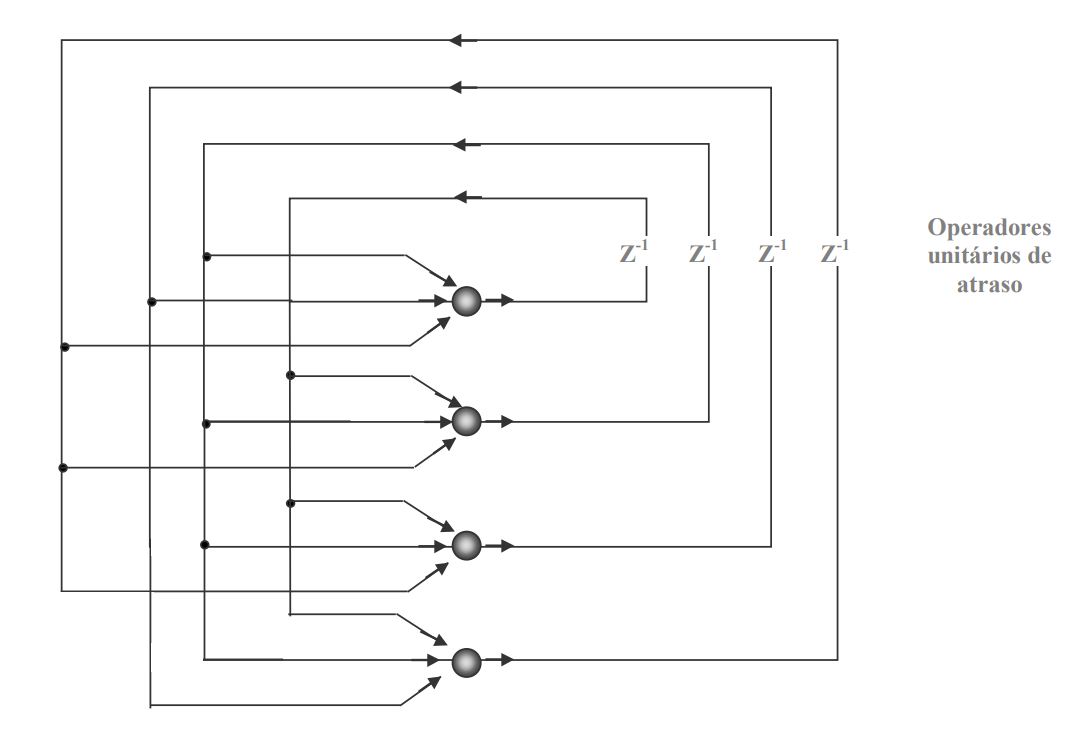
\includegraphics[width=.75\textwidth]{figuras/recorrente.png}
% \caption{Exemplo de rede neural artificial do tipo Recorrente ou Realimentada. [Imagem: \cite{furtado2019redes}]}
% \label{figredeRecorrente}
% \end{figure}

% \subsection{Treinamento}

% Após projetada a arquitetura da rede (determinar número de entradas, saídas, camadas escondidas e número de neurônios), é necessário um algoritmo de treinamento para realizar a aprendizagem da mesma. Para tal fim, é usualmente utilizada uma metodologia, em que a rede aprende acerca de seu ambiente a partir de um processo de ajustes sobre seus pesos sinápticos, isto é, os valores das sinapses são modificados aos poucos, visando minimizar os erros e otimizar a saída da rede. Idealmente, a rede se torna mais instruída sobre o seu ambiente após cada iteração do processo de aprendizagem \cite{haykin2011neural}.

% A arquitetura da rede define, dentre outros parâmetros, a que tipo de treinamento a rede será submetida, capacitando-a a resolver o problema. Segundo \cite{furtado2019redes}, os processos de aprendizagem podem ser agrupados em três paradigmas principais: aprendizado supervisionado, aprendizado não-supervisionado e aprendizado por reforço.

% Aprendizado supervisionado implica a existência de um supervisor ou professor, o qual é responsável por estimular as entradas da rede por meio de padrões de entrada e observar a saída da rede calculada pela mesma, comparando-a com a saída desejada

% O treinamento supervisionado utiliza um supervisor(professor), o qual é responsável por estimular as entradas da rede por meio de padrões de entrada e observar a saída da rede calculada pela mesma, comparando-a com a saída desejada. Através do erro, que é a diferença entre os valores esperados e os valores obtidos, o agente externo ajusta os parâmetros da rede. Este ajuste é feito até que o erro seja minimizado, passando a não existir mais ou atingindo um valor considerado satisfatório \cite{de2007redes}. 

% A partir deste momento, diz-se que a rede adquiriu conhecimento e apresenta-se treinada. Esse tipo de aprendizado é aplicado em problemas em que se deseja mapear padrões de entrada e saída. Dentre os algoritmos de treinamento supervisionado, pode-se citar como exemplo o do Erro Médio Quadrático e a generalização do mesmo, o backpropagation. Segundo \cite{haykin2011neural}, o backpropagation é o algoritmo de RNAs mais usado em aplicações práticas de previsão, classificação e de reconhecimento de padrões em geral. 

% No aprendizado não-supervisionado não existe um supervisor(professor) e em geral, apenas os padrões de entrada estão disponíveis, ou seja, não apresenta uma saída-alvo para comparação. Portanto, o processo de aprendizagem se dá pela existência de regularidades e redundâncias nos padrões de entrada apresentados à rede, a qual, deverá ser capaz de extrair as características relevantes dos impulsos, classificando-os em grupos pré-existentes. Esse processo se aplica em problemas que visam à descoberta de características estatísticas nos dados.

% O  aprendizado  por  reforço, mesmo  apresentando  similaridades  com  o  aprendizado supervisionado  e  não  supervisionado,  é  diferente,  pois  é  caracterizado  por haver  um supervisor que não indica uma saída desejada, apenas avalia se a saída está correta ou não. É um método baseado em tentativa e erro, pois os ajustes dos pesos a serem tomados irão depender unicamente das respostas produzidas pelo sistema durante o treinamento. O que o diferencia do treinamento supervisionado é que o supervisor sabe exatamente como ajustar os pesos no caso de erro.

% \subsection{Backpropagation}

% Este é um algoritmo de treinamento supervisionado para redes do tipo Feedforward
% que tenham neurônios com qualquer função de ativação que seja derivável. A ideia do algoritmo é estimar os valores dos pesos e bias minimizando o erro entre a entrada e a saída desejada usando o gradiente descendente. O erro \(E\) cometido pela rede é calculado por:

% \begin{equation} \label{eqRNA3}
% \begin{split}
% E = \frac{1}{2} \sum_{i=1}^{p} \sum_{j=1}^{n} (d_{j}^{i} - y_{j}^{i})^2
% \end{split}
% \end{equation}

% no qual, \(p\) é o número exemplos a ser utilizados no treinamento, n é o número de saídas da rede e, finalmente, \(d\) e \(y\) são as saídas desejadas e obtidas, respectivamente, para a entrada em questão.

% Se o erro \(E\) encontrado for retropropagado (termo que foi derivado do nome do algoritmo backpropagation) pela rede, isto é, se o erro for propagado a partir da camada de saída até a camada de entrada, ela tentará estabelecer o quanto cada sinapse contribuiu para o erro, e este será usado para ajustá-las. A regra de atualização de cada peso sináptico da rede é calculado pela seguinte equação:

% \begin{equation} \label{eqRNA4}
% \begin{split}
% W = W + \Delta W \therefore \Delta W = - \alpha\frac{\partial E}{\partial W}
% \end{split}
% \end{equation}

% onde, \(\alpha\) é conhecido como taxa de aprendizado, que, resumidamente, indica o ‘tamanho do passo’ do gradiente rumo a minimização. O sinal negativo indica a busca por uma alteração no peso que reduza \(E\), sendo assim, quanto menor o erro, melhor a rede estará mapeando o problema.

\chapter{Metodologia}

\section{Obtenção e Processamento dos Dados}

Tanto para o processo de treinamento quanto para o processo de teste de uma RNA, o primeiro passo a ser dado é a obtenção das amostras experimentais para o treinamento supervisionado e teste das RNAs. Algoritmos de maquina de aprendizado supervisionados são muito mais eficazes quando treinados com conjuntos de dados muito grandes.

O primeiro passo dado nesta pesquisa foi a coleta dos dados das GW. Em 1 de dezembro de 2018, o LIGO Scientific Collaboration e o Virgo Collaboration anunciaram o GWTC-1~\cite{Abbott_2019}, catálogo de GW observadas pelo LIGO e Virgo durante a primeira e a segunda execução de observações, contendo os resultados completos de suas pesquisas por GW, que conta com onze detecções de GW provenientes dez de sistemas binários de buracos negros e um sistemas binário de estrelas de nêutrons. Como as fusões de buracos negros dominam o número de detecções de GW, este trabalho focou exclusivamente neste tipo de detecção, as quais estão disponíveis no LIGO Open Science Center (LOSC)\footnote{\href{https://www.gw-openscience.org/about/}{ttps://www.gw-openscience.org/about/}}~\cite{vallisneri2015ligo}. 

Após a obtenção dos dados, foram analisados e selecionados nove das dez amostras de GW de fusão de buracos negros, sendo elas: GW150914, GW151012, GW151226, GW170104, GW170608, GW170729, GW170809, GW170814, GW170823. As quais foram processadas com a ajuda da ferramenta PyCBC\footnote{\href{https://pycbc.org/}{https://pycbc.org/}}~\cite{alex_nitz_2019_2801307}, que é um pacote de software escrito em Python\footnote{\href{https://www.python.org/}{https://www.python.org/}}, usado para explorar e analisar as fontes astrofísicas de GW, e capaz de detectar binários compactos coalescentes e medir seus parâmetros astrofísicos. O PyCBC contém diversos módulos para processamento de sinais e um deles é capaz de gerar formas de GW. A partir desse módulo foi gerado uma forma de GW equivalente ao formato real das GW capturados pelos detectores de GW (Hanford-H1 e Livingston-L1 Interferômetros) para cada uma das amostras selecionadas.

Devido aos detectores terem uma alta sensibilidade, ruídos de origens instrumentais, ambientais e provenientes de atividades humanas sempre o atingem, poluindo os sinais e dificultando as detecções. Durante todo o processo os dados oriundos do LIGO foram limpos e filtrados e também ignoradas as falhas, os blips e outras fontes de ruído de detectores transientes que dificultam a analise e processamento das GW.

As formas de GW são geradas como uma série temporal, usando uma das aproximações de forma de onda disponíveis pelo PyCBC. Os parâmetros principais foram as massas do sistema binário (dadas em massas solares), o tempo entre as amostras (em segundos), a frequência inicial das GW (Hz) e o nome do aproximante que gostaríamos de gerar. Está disponível uma variedade de aproximações que incluem diferentes efeitos físicos. A precisão numérica depende da resolução, enquanto a precisão da extrapolação pode ser avaliada pela comparação de diferentes ordens de extrapolação. Pedidos mais altos tendem a produzir melhores resultados na fase inspiral, mas pior na fase do ringdown \cite{scharpf2017simulation}. 

Desta forma optou-se por buscar aproximadores com níveis mais elevados de precisão que tivessem o melhor resultado para ambas as fases das simulações, devido a resultados mais atualizados e mais precisos. Para esta pesquisa foi usado o aproximante IMRPhenomD, pois atende altos níveis de precisão graças a uma combinação de métodos analíticos post-Newtonian (PN) e effective-one-body (EOB) para descrever a inspiração, e a calibração de modelos fenomenológicos de fusão-ringdown para simulações de relatividade numérica (NR)~\cite{khan2015frequencydomain}. Ele modela a forma de GW nas fases de inspiração, fusão e ringdown dos buracos negros e inclui a capacidade de cada buraco negro girar na mesma direção que a órbita (rotação alinhada), atingindo bons resultados em ambas as fases de inspiral e ringdown. Além de poderem ser geradas rapidamente e para uma ampla gama de valores de parâmetros.

O PyCBC foi usado no projeto descrito nesta tese tanto para geração de banco de modelos quanto todo o processo de filtragem correspondente dos dados brutos advindos do LIGO. Usamos o PyCBC para geração simples de GW no domínio da frequência com massas e tempo de amostras iguais as dos sistemas binários descritos no catalogo GWTC-1 com uma frequência inicial de 20Hz. Portanto, foram gerados dezoito GW equivalentes as GW detectadas pelo LIGO, nove para cada detector LIGO (Hanford-H1 e Livingston-L1).

A escolha e adequação dos dados utilizados para treinar e testar uma RNA é de fundamental importância. É necessário que se disponha de dados em quantidade e qualidade suficientes. Caso a quantidade de dados seja pequena, a rede não conseguirá criar um modelo suficientemente representativo para se ter um desempenho satisfatório quando aplicado em situações reais após o seu desenvolvimento, o que é chamado de sobre-ajuste (overfitting) dos dados. Além disto, os dados devem englobar todos os aspectos do problema em questão, a fim de que o modelo criado seja genérico. 

Como o objetivo é treinar uma RNA que forneça um diagnóstico classificativo entre GW e Ruído, que apresente um bom desempenho, extraímos um intervalo de 0.1 segundos de cada forma de onda com pico centralizado, deslocando a localização de pico de cada sinal aleatoriamente dentro de um intervalo de 0 a 0.05 segundos para a direita, a uma taxa de amostragem de 4096Hz. Este processo foi repetido 600 vezes para cada uma das formas de onda geradas, criando assim 10800 modelos de GW, a Figura~\ref{fig:gw150914-offset} ilustra algumas das ondas geradas.

\begin{figure}[ht]
    \centerline{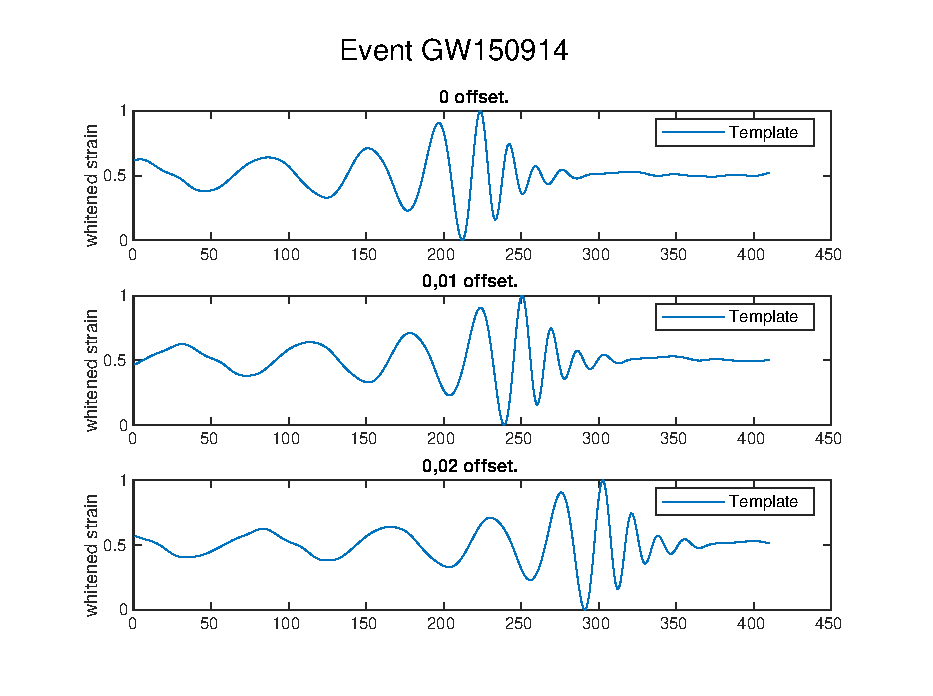
\includegraphics[width=1\textwidth]{figuras/GW150914.eps}}
    \caption{Alguns modelos de GW com deslocamento}
    \label{fig:gw150914-offset}
\end{figure}

Os modelos de machine learning são construídos para minimizar erros. Desde que a probabilidade pertence a classe com maior número de observação, o algoritmo estará enviesado em classificar as novas observações. Afim de evitar o enviesamento por causa do desbalanceamento dos dados, foi criado também a mesma quantidade de amostras de ruído com espectro equivalente a densidade espectral de potência (DEP ou PSD em inglês) do ruido do LIGO~\cite{T1800044}. No final da construção dos dados, juntamos os dois bancos de dados (ruídos e ondas), totalizando o conjunto de dados de treinamento, teste e validação com um total de 21600 amostras com duas classes: Ondas e Ruídos.

É esperado que uma RNA, após a fase de treinamento, seja capaz de produzir respostas corretas a estímulos externos, mesmo que estes não sejam exatamente iguais aos estímulos utilizados no seu treinamento. Para o conjunto de dados de novos estímulos, foram necessários 2.0 segundos de observação a uma taxa amostral de 4096Hz de cada um das nove GW selecionadas anteriormente, filtradas com a onda centralizada, na qual eles foram separados em várias janelas de 0.1 segundos (410 pontos) com passos de uma unidade e a mesma taxa de frequência amostral, gerando assim aproximadamente ~7780 janelas de dados. Esses dados foram gerados para os dois detectores LIGO (Hanford-H1 e Livingston-L1) separadamente, totalizando aproximadamente ~140000 de dados.

Alguns algoritmos têm dificuldade em entender variáveis que têm mais do que uma categoria. Pelo fato dos dados apresentarem duas classes categóricas (onda e ruído) o algoritmo de Machine Learning que empregamos nesta pesquisa não produz bons resultados com esses dados categóricos. Diante dessa limitação foi preciso converter as variáveis categóricas para valores numéricos. Buscando melhorar o processamento dos dados foi aplicado uma técnica de pré-processamento de dados chamada one-hot encoding. 

O one-hot encoding é usada em Machine Learning como um método para quantificar dados categóricos e melhorar significativamente os resultados \cite{sarkar2017practical}. Em resumo, esse método produz um vetor com comprimento igual ao número de categorias no conjunto de dados. Neste caso, as classes onda e ruído são transformadas em vetores como: $[1,0]$ e $[0,1]$ respectivamente, que indicam a saída correspondente desejada da RNA para cada uma das classes do conjunto de dados.

Com essa imensa quantidade de dados seria difícil manter tudo sobre estruturas de arquivos simples como ".csv", pois além de consumir muito espaço físico o processo de leitura desses arquivos se tornaria demasiadamente longo. Para resolver este problema, todos os conjuntos de dados foram salvos em HDF (Hierarchical Data Format), que é uma biblioteca de software e formato de dados de alto desempenho (HDF4, HDF5) projetados para armazenar e organizar grandes quantidades de dados para facilitar a leitura dessa grande massa de dados~\cite{hdf}. Por usar árvores B para indexar os dados, o HDF funciona bem para dados de séries temporais. A maior parte dos dados entra em matrizes simples que podem ser acessadas muito mais rapidamente do que as linhas de um banco de dados SQL. 

O HDF foi desenvolvido para processamento e armazenamento de E/S rápidos de alto desempenho com um rico conjunto de recursos de desempenho integrados que permitem otimizações de tempo de acesso e espaço de armazenamento~\cite{hdf}. Esta biblioteca foi amplamente adotada em vários setores e é o padrão de fato na comunidade científica e de pesquisa, uma vez que a maioria das ferramentas que usa Machine Learning suportam esse tipo de arquivo.

\section{Arquitetura da Rede Neural}

Definir a arquitetura de uma RNA é muito importante devido ao fato de que seu arranjo depende do problema a ser tratado pela rede. Ademais, a arquitetura da rede está intimamente relacionada ao algoritmo de aprendizagem usado para treinamento. De acordo com o teorema da aproximação universal, aplicado às redes MLP, uma única camada escondida de neurônios é suficiente para realizar uma aproximação de qualquer função contínua para um dado conjunto de treinamento representado pelo conjunto de entradas e a saídas-alvo\cite{cybenko1989approximation, haykin2007redes}. O uso de mais camadas pode reduzir o tempo de treinamento da rede e possibilitar que um número menor de neurônios seja suficiente para que a rede atinja o desempenho esperado.~\cite{daredes}.

% Porém, o teorema não diz que uma única camada oculta terá uma solução ótima, além de não prever a quantidade de neurônios necessários para a aproximação adotada. Ou seja, trata-se de um teorema existencial, o qual justifica matematicamente a aproximação de uma função contínua arbitrária por uma rede perceptron de uma camada oculta. Dessa forma, a comparação entre as três arquiteturas adotadas ilustrará as capacidades e limitações de cada uma.

Com base nesta premissa, foi usado uma arquitetura de RNA simples para otimizar e acelerar o processo de treinamento e detecção de GW. Foi gasto um tempo significativo pesquisando por tentativa e erro uma ótima arquitetura de RNA e otimizando hiperparâmetros. Após sucessivas simulações para determinação do número de entradas das redes neurais, foi estabelecido que a rede neural teria 410 entradas. Sendo assim, cada janela de dados das GW seria apresentados à rede, ou seja, o classificador será aplicado ao fluxo de dados contínuo usando janelas deslizantes de 0,1 segundo de largura com uma diferença de 200 microssegundos.

Diversas estruturas de RNA do tipo MLP com diferentes quantidades de neurônios na camada escondida e diferentes funções de ativação foram testadas visando obter a melhor e mais otimizada estrutura MLP a ser empregada nesta dissertação para a detecção de GW. Essa estrategia de testar varias estruturas é a prática mais recomendada e aprovada quando se deseja escolher a estrutura mais adequada para algum problema~\cite{OKOH201619}.

No entanto, foi possível aprimorar ainda mais a discriminação da RNA graças a implementação do one-hot encoding, que definiu duas categorias quantizadas representadas pelos valores binários de 0 e 1 e consequentemente a RNA acompanhou a quantidade de saída desejada e foi colocado duas saídas na última camada da RNA, as saídas A e B. 

Agora, por exemplo, se o estimulo de entrada da rede fosse da classe "Onda", as saídas da RNA desejadas seriam A = 1 e B = 0 [1,0] e se o estimulo de entrada fosse da classe "Ruído", as saídas da RNA desejadas seriam A = 0 e B = 1 [0,1]. Com essas duas saídas, é possível definir um score como:

\begin{equation}
score = \frac{a-b}{2}+0.5
\label{eq:score}
\end{equation}

Dessa forma, a saída da RNA desejada para a classe Onda terá uma pontuação que tenderá a 1 ($score \rightarrow 1$), e a saída da RNA desejada para a classe Ruído terá uma pontuação que tenderá a 0 ($score \rightarrow 0$). 

Durante o processo de encontrar a melhor estrutura e parâmetros para a rede, o modelo foi avaliado através de uma análise de distribuição dos resultados, do erro quadrático médio (MSE) e do cálculo da estatística de Kolmogorov-Smirnov (KS). Graças ao score desenvolvido na equação \ref{eq:score}, foi possível construir uma distribuição de pontuação para cada classe, e a capacidade de discriminação da RNA pode ser medida com o uso da distância KS. Essa distância KS é a distância máxima entre duas funções de distribuição cumulativa empírica (ECDF), que quando normalizadas são um valor na faixa [0,1]. O KS é descrito pela teoria estatística não paramétrica e é utilizada para testar se as distribuições de dois grupos são iguais~\cite{daniel2000applied}. 

O teste de KS tem sido utilizado para avaliar o desempenho de classificadores binários avaliando a diferença entre as distribuições dos maus e bons clientes \cite{karcher2009redes} e distribuição do cliente mais propensos a quitar suas dividas ou não \cite{forti2018tecnicas}  por exemplo, neste caso, quanto maior for a estatística de KS, maior será a separação entre os clientes adimplentes e inadimplentes como também entre cliente quitados e não quitados respectivamente. 

Em outras palavras, para esta pesquisa ele avalia o quão bem o modelo consegue distinguir os classificados como Onda dos classificados como Ruído. Sendo assim, o KS se comporta como uma medida de avaliação de performance, quanto maior for o resultado do KS (indicação de maior diferença entre as distribuições), melhor está a acurácia do modelo, pois a separação das classes é maior. 

A estatística de Kolmogorov–Smirnov pode ser descrita por: 
\begin{equation}
KS = Max|F1(x)−F2(x)|
\label{eq:kolmogorov}
\end{equation}

Onde Max é a maior distância entre as distribuições de F1 e F2, em que, F1 é a distribuição acumulada do score dos classificados como Ondas e F2 é a distribuição acumulada do score dos classificados como Ruído.

A Figura~\ref{fig:ANN_Distribution_a} mostra uma ilustração pictórica da distribuição empírica do score gerado para o problema de classificação binária, onde a classe $X$ tem uma distribuição do score centrada em torno de $0$ e a classe $Y$ tem uma distribuição do score em torno de $1$. A Figura~\ref{fig:ANN_Distribution_b} apresenta a distância KS entre essas duas distribuições.

\begin{figure}[H]
\centering
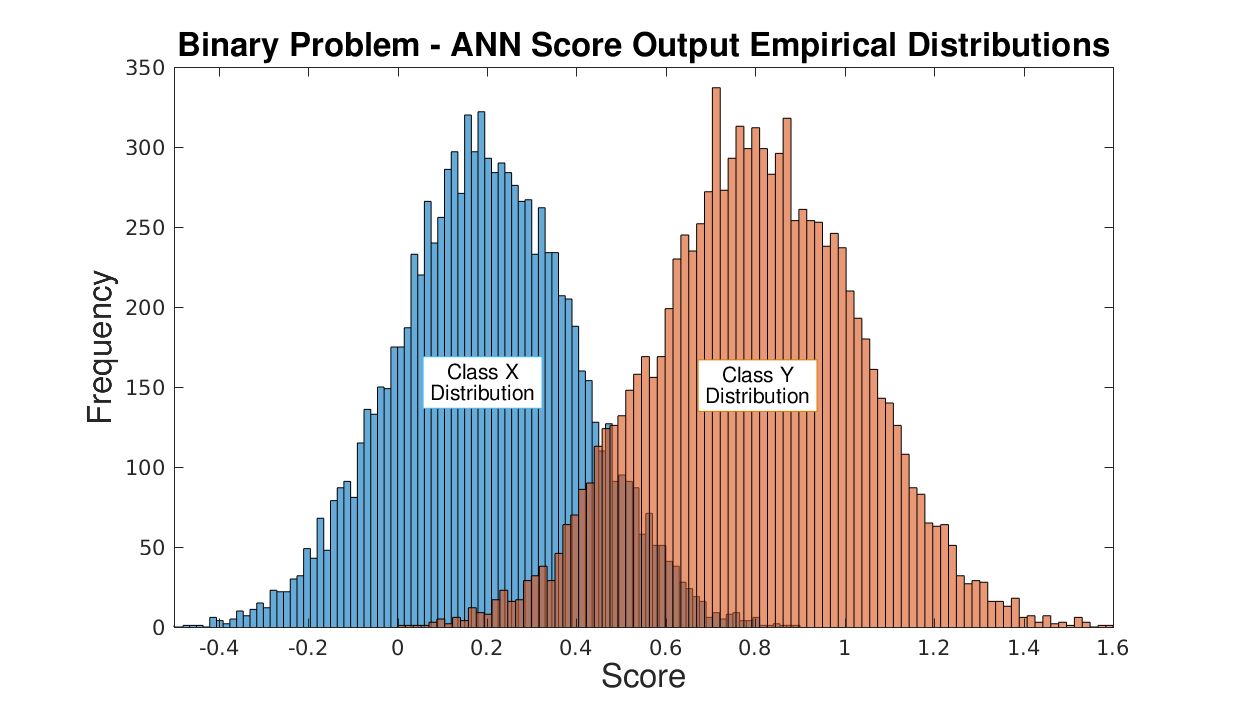
\includegraphics[width=1\textwidth]{figuras/ANNScore_Output.eps}
\caption{Resposta pictórica do score da RNA para um problema de classificação binária - Distribuição empírica do score.}
\label{fig:ANN_Distribution_a}
\end{figure}

\begin{figure}[H]
\centering
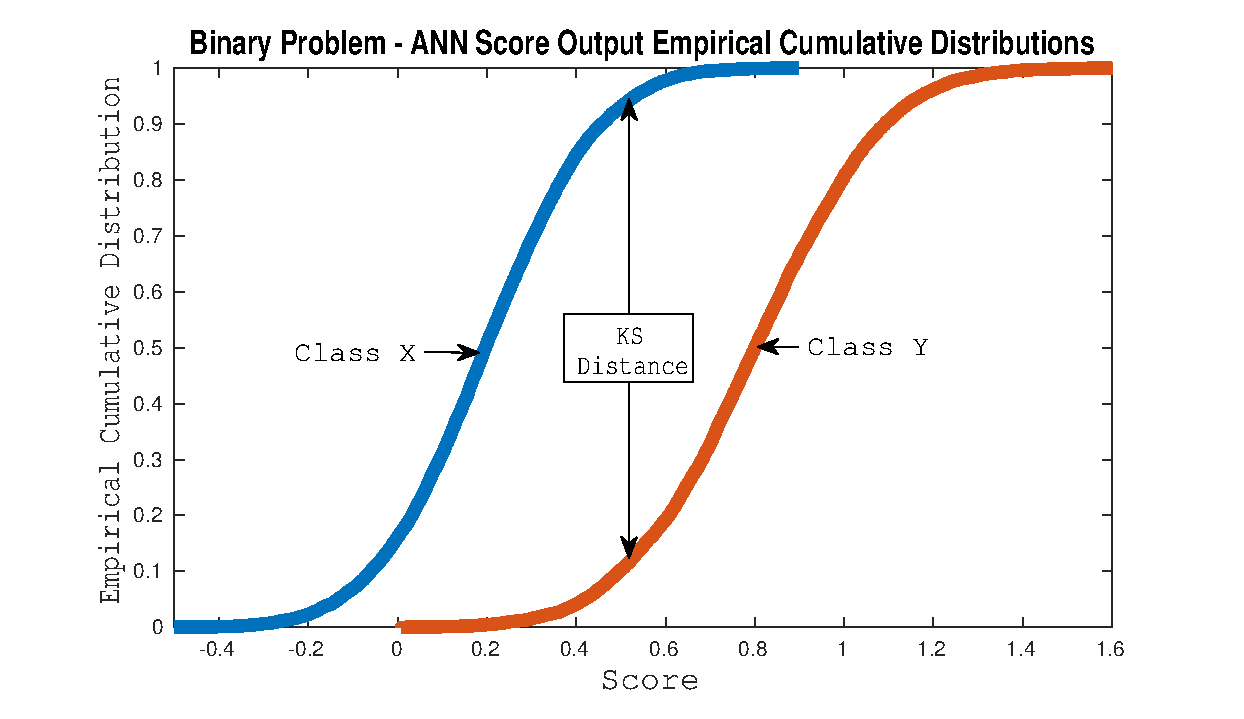
\includegraphics[width=1\textwidth]{figuras/ANNScore_Output_Cumulative.eps}
\caption{Resposta pictórica do score da RNA para um problema de classificação binária --- Distribuição empírica do score acumulada.}
\label{fig:ANN_Distribution_b}
\end{figure}

\section{Treinamento da Rede}

O principal objetivo do processo de aprendizagem de uma RNA é fazer com que um conjunto de entradas produza um conjunto de saídas desejadas ou, no mínimo, um conjunto de saídas aceitável, ao serem aplicadas em uma RNA~\cite{haykin2007redes}.

Para uma RNA, o conceito de treinamento diferencia-se do conceito de aprendizado. O aprendizado está associado a uma tarefa que a rede está executando em função do treinamento e da sua modelagem. Já o treinamento é o processo de ensinar a RNA~\cite{furtado2019redes}.

Pode-se dizer que o treinamento da rede neural é o ponto mais critico que determina o desfecho da rede, pois, neste procedimento, a rede é submetida ao aprendizado, onde alguns fatores dos parâmetros de treinamento são relevantes, como: o algoritmo de treinamento, o número máximo de iterações, a taxa de aprendizagem, a função de ativação e muitos outros.

A seleção dos parâmetros de treinamento de uma RNA pode ser um processo complexo, pois pequenas diferenças nestes parâmetros podem levar a grandes diferenças tanto no tempo de treinamento como na generalização obtida. É um processo tão pouco compreendido que é muitas vezes é chamado de “magia negra”.

Nesta pesquisa foi usado o paradigma de aprendizagem supervisionado com o algoritmo Backpropagation em todas as redes. Para sua utilização, alguns parâmetros inerentes do algoritmo precisaram ser definidos. Algumas heurísticas também foram adotadas com o intuito de aumentar o desempenho do processo de aprendizagem e aumentar a eficiência do modelo.

A taxa de aprendizagem tem grande influência durante o processo de treinamento da
rede neural. Uma taxa de aprendizado muito baixa torna o aprendizado da rede muito lento, à medida que uma taxa de aprendizado muito alta provoca oscilações no treinamento e impede a
convergência do processo de aprendizado. Desta forma, seu valor inicial variou de 0.1 a 1.0, mas este parâmetro foi definido como adaptativo, por isso a escolha de um valor inicial não resultou em um grande problema. 

O número máximo de iterações (épocas) foi determinado para evitar o overfitting da rede. Um número excessivo de épocas pode levar a rede à perda do poder de generalização (overfitting). Por outro lado, com um pequeno número de épocas a rede pode não chegar ao seu melhor desempenho (underfitting). Diferente da taxa de aprendizagem o numero de épocas se manteve constante durante toda a pesquisa e foi definido com 100000 épocas. Contudo, mesmo sendo um número grande, este parâmetro foi usado como critério de parada no processo de treinamento das redes.

As funções de ativação são um elemento de extremamente importante das RNAs. Elas basicamente decidem se um neurônio deve ser ativado ou não. Ou seja, se a informação que o neurônio está recebendo é relevante e deve ser propagada ou não~\cite{DeepLearningBook}. Para que se encontrasse a função de ativação que melhor se adequasse as redes desenvolvidas nesta pesquisa, foram usadas somente três funções de ativação, são elas: Linear, Sigmoide e Tangente Hiperbólica.

Uma das dificuldades processo de treinamento de uma RNA consiste em encontrar o melhor ponto de parada do treinamento, pois o erro de treinamento começa com um valor muito alto, decai rapidamente, e continua diminuindo lentamente, tendendo a atingir um mínimo local na superfície de erro~\cite{haykin2007redes}. Para isto, existem vários métodos para a determinação do momento em que o treinamento de uma RNA deve ser encerrado. Uma boa determinação deste momento é fundamental para um bom treinamento e consequentemente uma boa generalização. Portanto, o treinamento é interrompido quando a rede apresenta uma boa capacidade de generalização e quando a taxa de erro é pequena, menor que um erro aceitável. É necessário encontrar um ponto ótimo de parada com o menor erro possível e capacidade de generalização máxima~\cite{barros2018avaliaccao}.

Neste sentido, o critério de parada no processo de treinamento não é bem definido e não há também uma convergência garantida. Geralmente é utilizado um número máximo de iterações, a taxa de erro médio por época e sua capacidade de generalização. Então, foi estipulado como método de parada para todas as RNAs desenvolvidas nesta pesquisa uma combinação de todos os métodos citados. Desta forma, o treinamento é encerrado quando qualquer um dos critérios é atendido.

Em relação aos pesos sinápticos, eles foram inicializados com números randômicos, mantendo o cuidado de não serem grandes suficientes para saturarem os neurônios, nem pequenos a ponto de atrasarem o aprendizado.

Para o conjunto de dados, normalmente são separados em dois conjuntos: conjunto de treinamento, que é usado para treinar a rede e conjunto de teste, que é utilizado para verificar a performance da rede sob condições reais de utilização. 

Afim de evitar o problema de overfitting, foi feita um subdivisão do conjunto de treinamento, criando um conjunto de validação, usado para verificar a eficiência da rede quanto a sua capacidade de generalização durante o processo de treinamento, o que se justifica o seu uso como critério de parada do treinamento da rede (taxa de erro médio).

O conjunto de dados de treinamento contém exatos 21600 amostras de dados. Desses dados, 70\% são para treinamento, 15\% para validação e 15\% para teste. O conjunto de dados reais para execução contém aproximadamente ~140000 dados, que são usados para a resolução final da rede executando situações reais com a rede treinada.

Depois de determinar estes conjuntos, eles foram colocados em ordem aleatória para prevenção de tendências associadas à ordem de apresentação dos dados. Além disso, foi necessário pré-processar estes dados, através de normalizações, para torná-los mais apropriados à sua utilização na rede. Todos os valores de entrada de todos os casos foram normalizados entre [0,1].

\section{Construção do Comitê}

A grande disponibilidade de recursos computacionais, possibilitou a criação de múltiplas propostas de soluções, as quais foram descartadas como testes e ajustes dos parâmetros para a busca do melhor modelo (rede). Entretanto, visto que, em certo ponto da pesquisa as RNAs descartadas apresentavam um desempenho parecido e com resultados consistentes, foi possível melhorar muito mais a capacidade de generalização do classificador implementando um comitê de redes neurais.

Para melhorar o processo de classificação ainda mais, várias RNAs com a melhor configuração foram treinadas. Dentre elas foram selecionadas 500 modelos com o melhor desempenho e esses formaram uma máquina de comitê que melhora significativamente os resultados. Graças a combinação do conhecimento adquirido pelas RNAs para chegar a uma solução global que é supostamente superior àquela obtida por qualquer RNA única~\cite{haykin1994neural}. 

A máquina do comitê desenvolvida na Figura~\ref{fig:comite} mostra um número k, em que k = 500 RNAs treinadas individualmente de maneira independente que compartilham uma entrada comum e cuja saída individual é de alguma forma combinada. para produzir uma saída geral. As saídas dessas redes são colocadas em um módulo de combinação que executa a função de calcular a média das saídas combinadas de todas as RNAs do comitê e apresentar o resultado semifinal do comitê de RNA.

\begin{figure}[H]
\centering
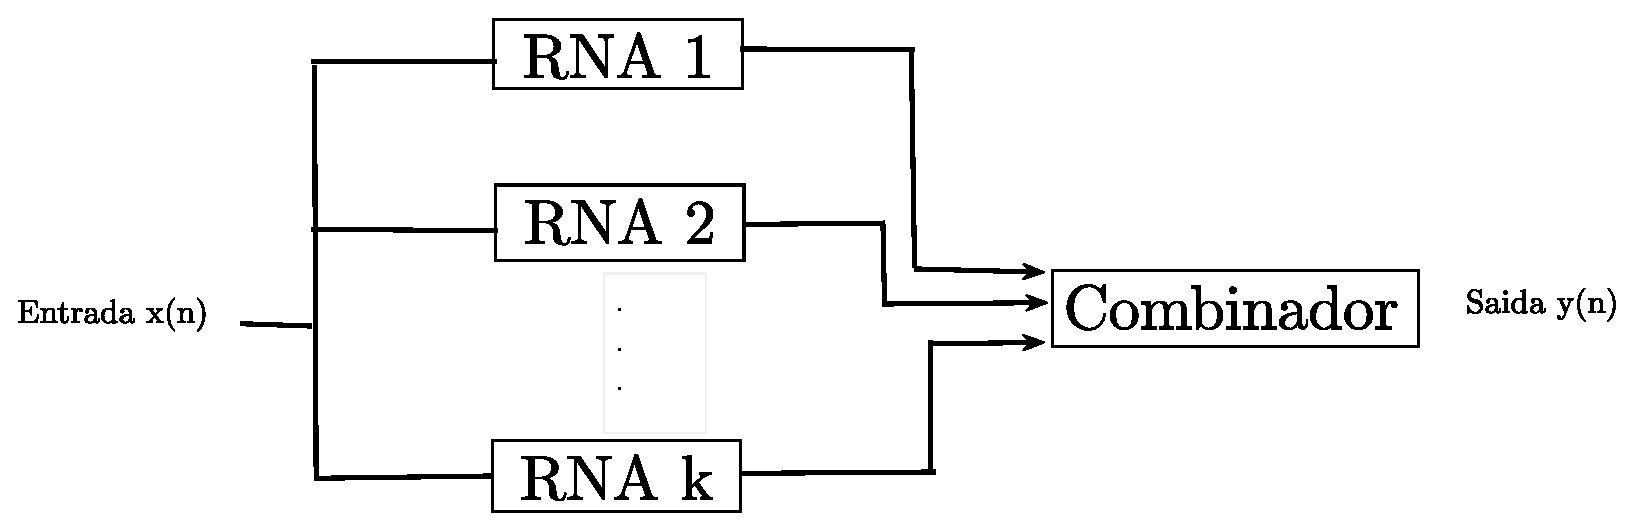
\includegraphics[width=1\textwidth]{figuras/comite.eps}
\caption{Diagrama de blocos de uma máquina de comitê.}
\label{fig:comite}
\end{figure}

Para implementação, execução e teste das RNAs, o software Matlab® R2018b\footnote{\href{ https://www.mathworks.com/products/matlab.html} {https://www.mathworks.com/products/matlab.html}} foi escolhido. Por possuir uma interface gráfica de treinamento de redes neurais, esse aplicativo suporta os mais diversos tipos de algoritmos de treinamento de redes neurais, permitindo que se possa executar uma extensa árvore de testes na tentativa de definir o modelo neural mais adequado, além de seu amplo uso pela comunidade científica.
\chapter{Resultados}

Foram realizados vários testes para encontrar o melhor modelo(rede) que atendessem os objetivos desta pesquisa, e após todo esse processo inicial, foi possível encontrar e definir os parâmetros da estrutura da RNA conforme é ilustrado na Figura \ref{fig:arquiteturarede}.

\begin{figure}[H]
\centering
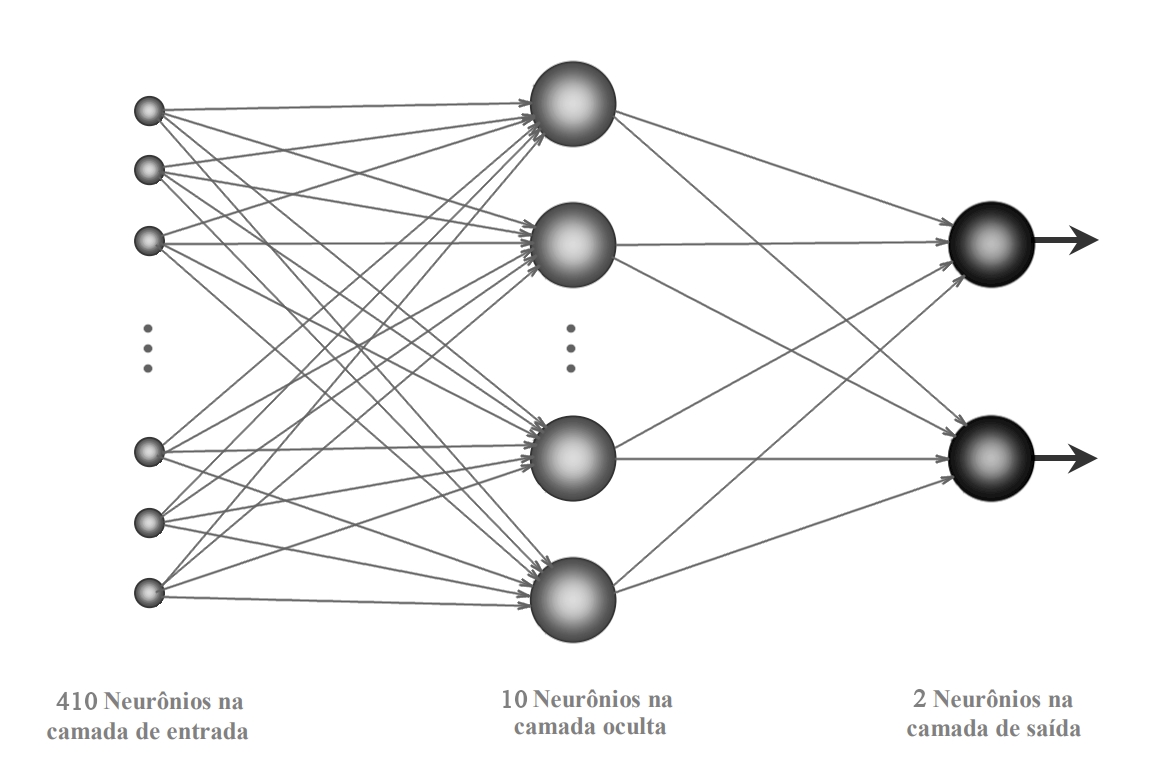
\includegraphics[width=1\textwidth]{figuras/arquitetura_rede.png}
\caption{Arquitetura da RNA.}
\label{fig:arquiteturarede}
\end{figure}

Como é mostrado na Figura \ref{fig:arquiteturarede}, a rede apresenta a configuração de 410 entradas, pois, as entradas foram restringidas a uma duração de 0,1 segundos, e a uma taxa de amostragem de 4096Hz.

Durante o processo de testes a configuração que obteve o melhor resultado foi com uma camada oculta contendo 10 neurônios. A quantidade pequena de neurônios foi suficiente para conseguir a generalização máxima, para o problema da pesquisa. Notou-se que durante o processo de testes o aumento da quantidade de neurônios na camada oculta prolongava o treinamento e influenciava negativamente na generalização da RNA. Para manter uma RNA de baixo custo computacional optou-se pela menor quantidade de neurônios sem perda de generalização do processo, o que resultou em uma RNA extremamente leve em comparação a redes neurais profundas. 

A camada de saída se manteve constante com 2 neurônios, devido ao método adotado na pesquisa, que utilizou da Equação~\ref{eq:score} para aprimorar a discriminação do resultado da RNA. Isto possibilitou a geração de duas distribuições do \textit{score}, uma para os classificados como Onda e uma para os classificados como Ruído.

E quanto aos parâmetros de treinamento, o número máximo de iterações permaneceu o mesmo durante toda a pesquisa com 100000 iterações, apesar de que, em nenhum momento a rede atingiu esse limite, mesmo assim foi usado como critério de parada. O valor inicial para a taxa de aprendizado foi de 0,025 mas foi usado uma taxa adaptativa. A função de ativação na camada oculta foi a Logarítmica Sigmoide, a qual, é comumente utilizada por redes neurais com propagação positiva (Feedforward) que precisam ter como saída apenas números positivos, em redes neurais multicamadas. A função de ativação usada na camada de saída foi a Linear, pois, apresentou melhor resultado dado que esta função não altera a saída do neurônio. Em consequência do uso da Equação~\ref{eq:score}  a função de ativação Softmax não foi cogitada, apesar de ser comumente usada em redes neurais de classificação.

Tanto o MSE quanto o KS foram utilizados como critério para definir a acurácia da rede, pois quanto menor o MSE melhor o resultado da RNA. Neste sentido a rede que apresentou o menor erro (MSE) possível, obtendo somente 0.000140842 de erro em apenas 5612 épocas de treinamento.

Consequentemente a RNA apresentou uma excelente discriminação das classe Onda e Ruído. É mostrado na Figura~\ref{fig:histograma} a distribuição do score gerado pela RNA, em que, a classe Onda tem uma distribuição do score centrada em torno de $1$, enquanto a classe Ruído tem uma distribuição do score em torno de $0$. 

\begin{figure}[H]
\centering
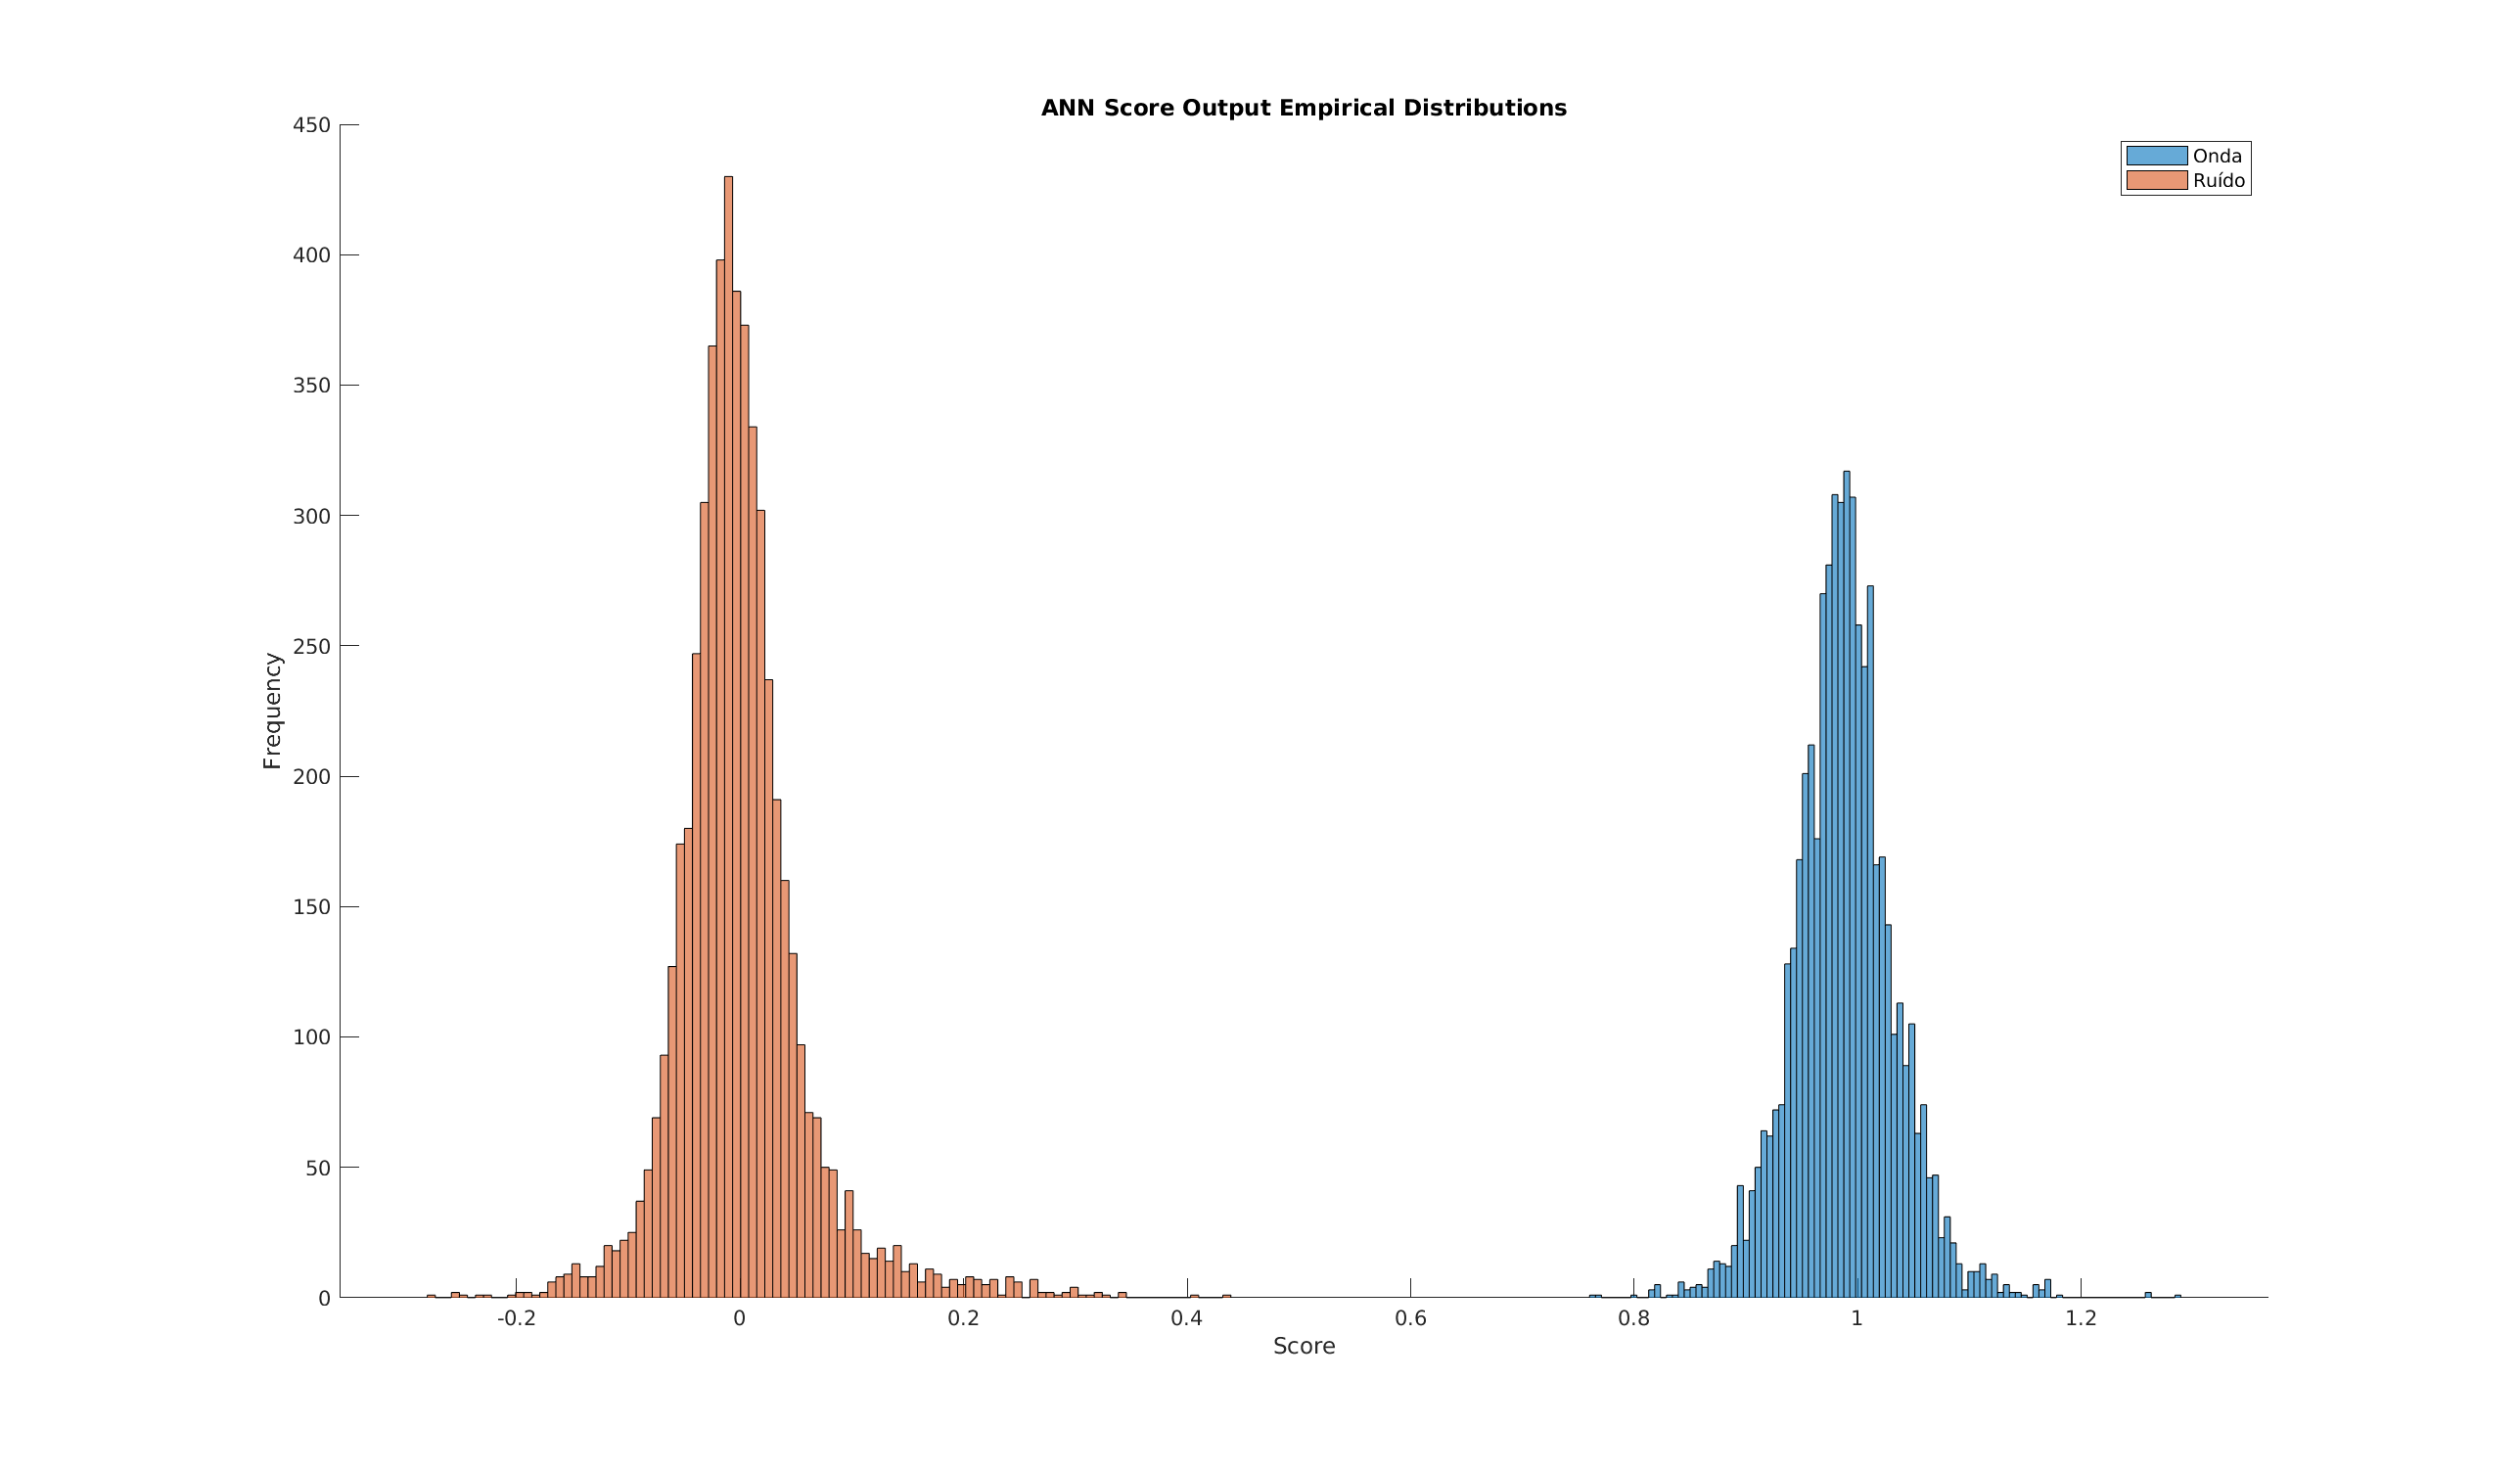
\includegraphics[width=1\textwidth]{figuras/histograma.eps}
\caption{Score da RNA para as duas classes (Onda e Ruído) - Distribuição empírica do score.}
\label{fig:histograma}
\end{figure}

É mostrado na Figura~\ref{fig:KS} a distância KS entre essas duas distribuições. É notável ver a separação das duas classes, pois, as distribuições não tem ponto de intersecção em comum. Portanto, o modelo distingue perfeitamente o que é um Onda Gravitacional tanto quanto o que é Ruído. Como a separação das duas distribuições foi muito evidente, o valor do KS assume o valor máximo de 1.

\begin{figure}[H]
\centering
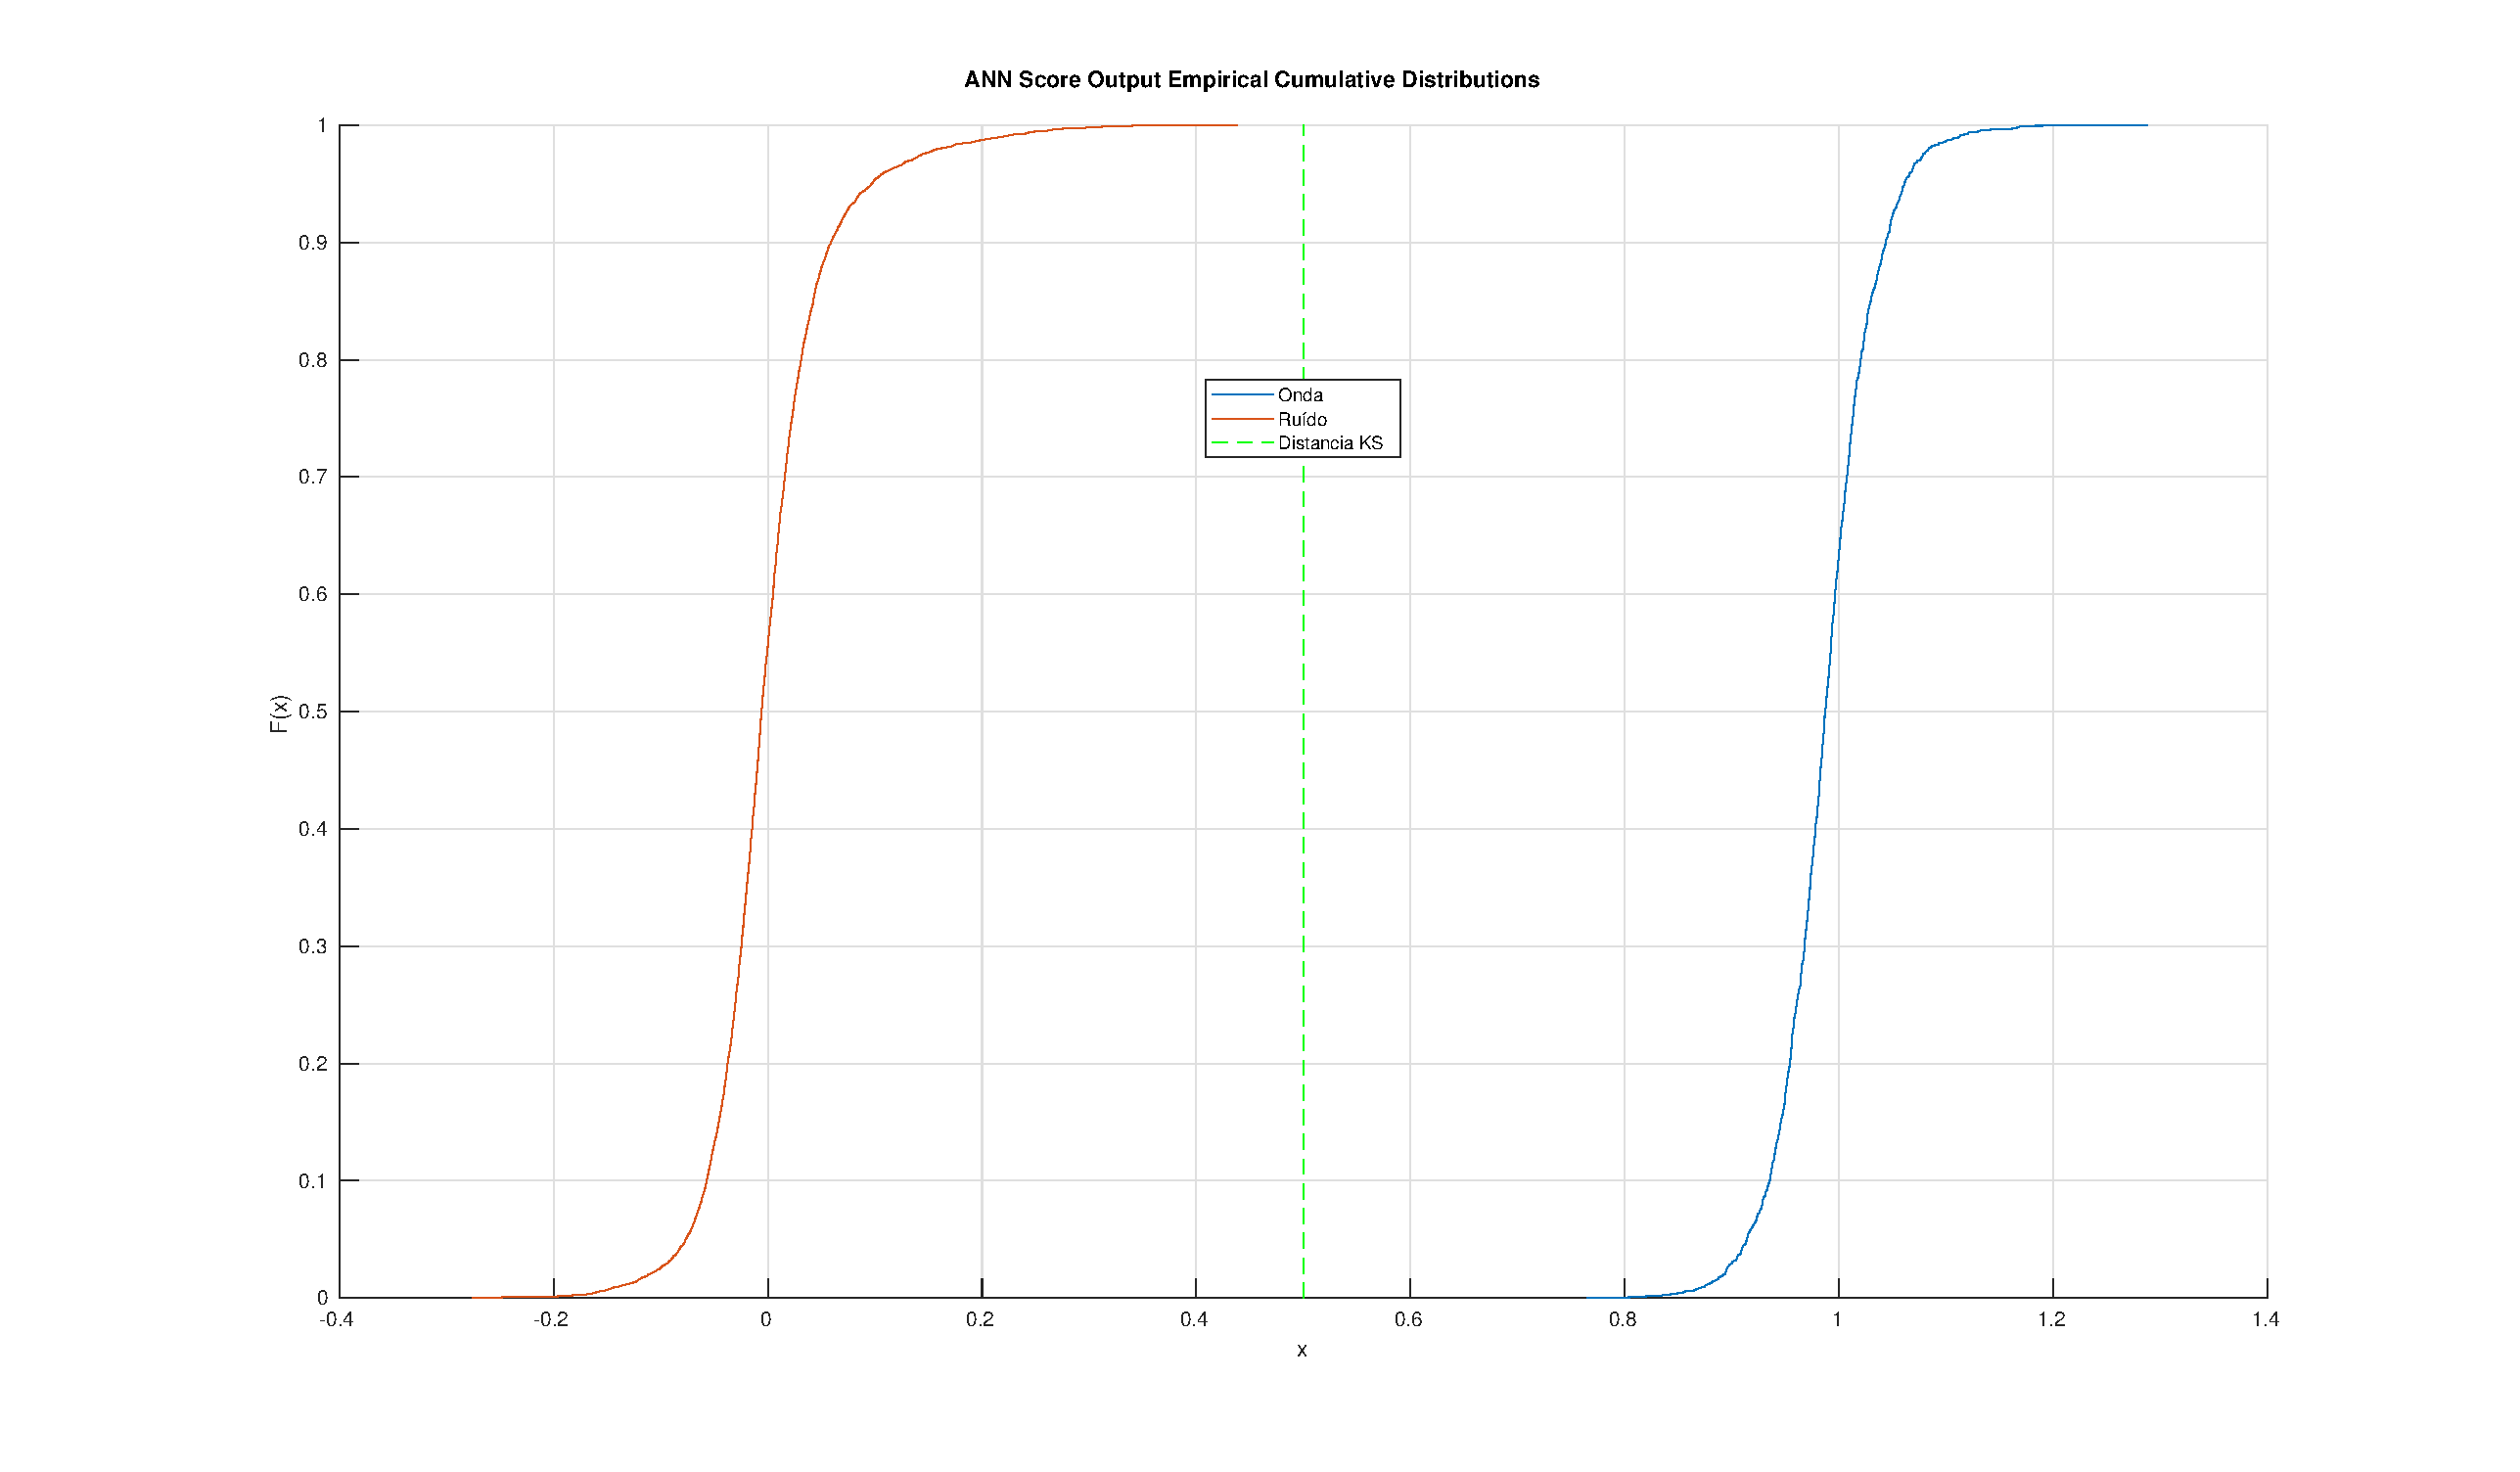
\includegraphics[width=1\textwidth]{figuras/KS.eps}
\caption{Score da RNA para as duas classes (Onda e Ruído) - Distribuição acumulada empírica do score.}
\label{fig:KS}
\end{figure}

Logo após encontrar o melhor modelo o comitê de RNA foi formado com as 500 melhores redes conforme é mostrado na Figura~\ref{fig:comite}. O critério de seleção das RNAs para o comitê, deu-se somente pelo MSE, dado que, todas as rede com a configuração descrita acima apresentam uma discriminação excelente como foi comprovado pelas Figuras~\ref{fig:histograma} e~\ref{fig:KS}.

Depois disso, quando o comitê recebeu os dados reais do LIGO para análise, um valor de score foi gerado. Foi gerado um score para cada um dos observatórios (H1 e L1) do LIGO para cada uma das nove ondas selecionadas.

Existem duas formas de analisar esse valor do score. Na primeira metodologia, na fase de treinamento, é determinado um valor de pontuação limite, em que valores inferiores a esse limite serão classificados como classe "Ruído" e valores maiores que esse limite serão classificados como classe "Onda". 

A segunda metodologia é considerar a distribuição empírica do score como uma função de pertinência. Assim, o valor do score pode ser visto como um termômetro, onde valores baixos do score implicam na classe ``Ruído" e valores altos do score na classe ``Onda".

Neste sentido esta pesquisa adotou a segunda metodologia a qual trata o score como um termômetro de ondas gravitacionais. Portanto o conjunto criado de dados reais do LIGO e separados em janelas deslizantes, produz resultados de um score ao longo do tempo, a medida que a janela deslizante percorre os dados.

É mostrado na Figura~\ref{fig:detection} o resultado após a rede ser submetida aos dados da onda gravitacional GW150914 do laboratório Hanford(H1). Nesta imagem é possível notar o valor do score ao longo do tempo, em que, em certo ponto o score cresce a medida que a janela deslizante apresenta a onda gravitacional ao classificador, até o ponto em que o score atinge o valor 1, onde a janela deslizante esta centrada na onda gravitacional. Por outro lado, quando a janela deslizante avança e a onda gravitacional sai do foco e é finalizada o score volta a se aproximar de zero e permanece próximo até o final da classificação.

\begin{figure}[H]
\centering
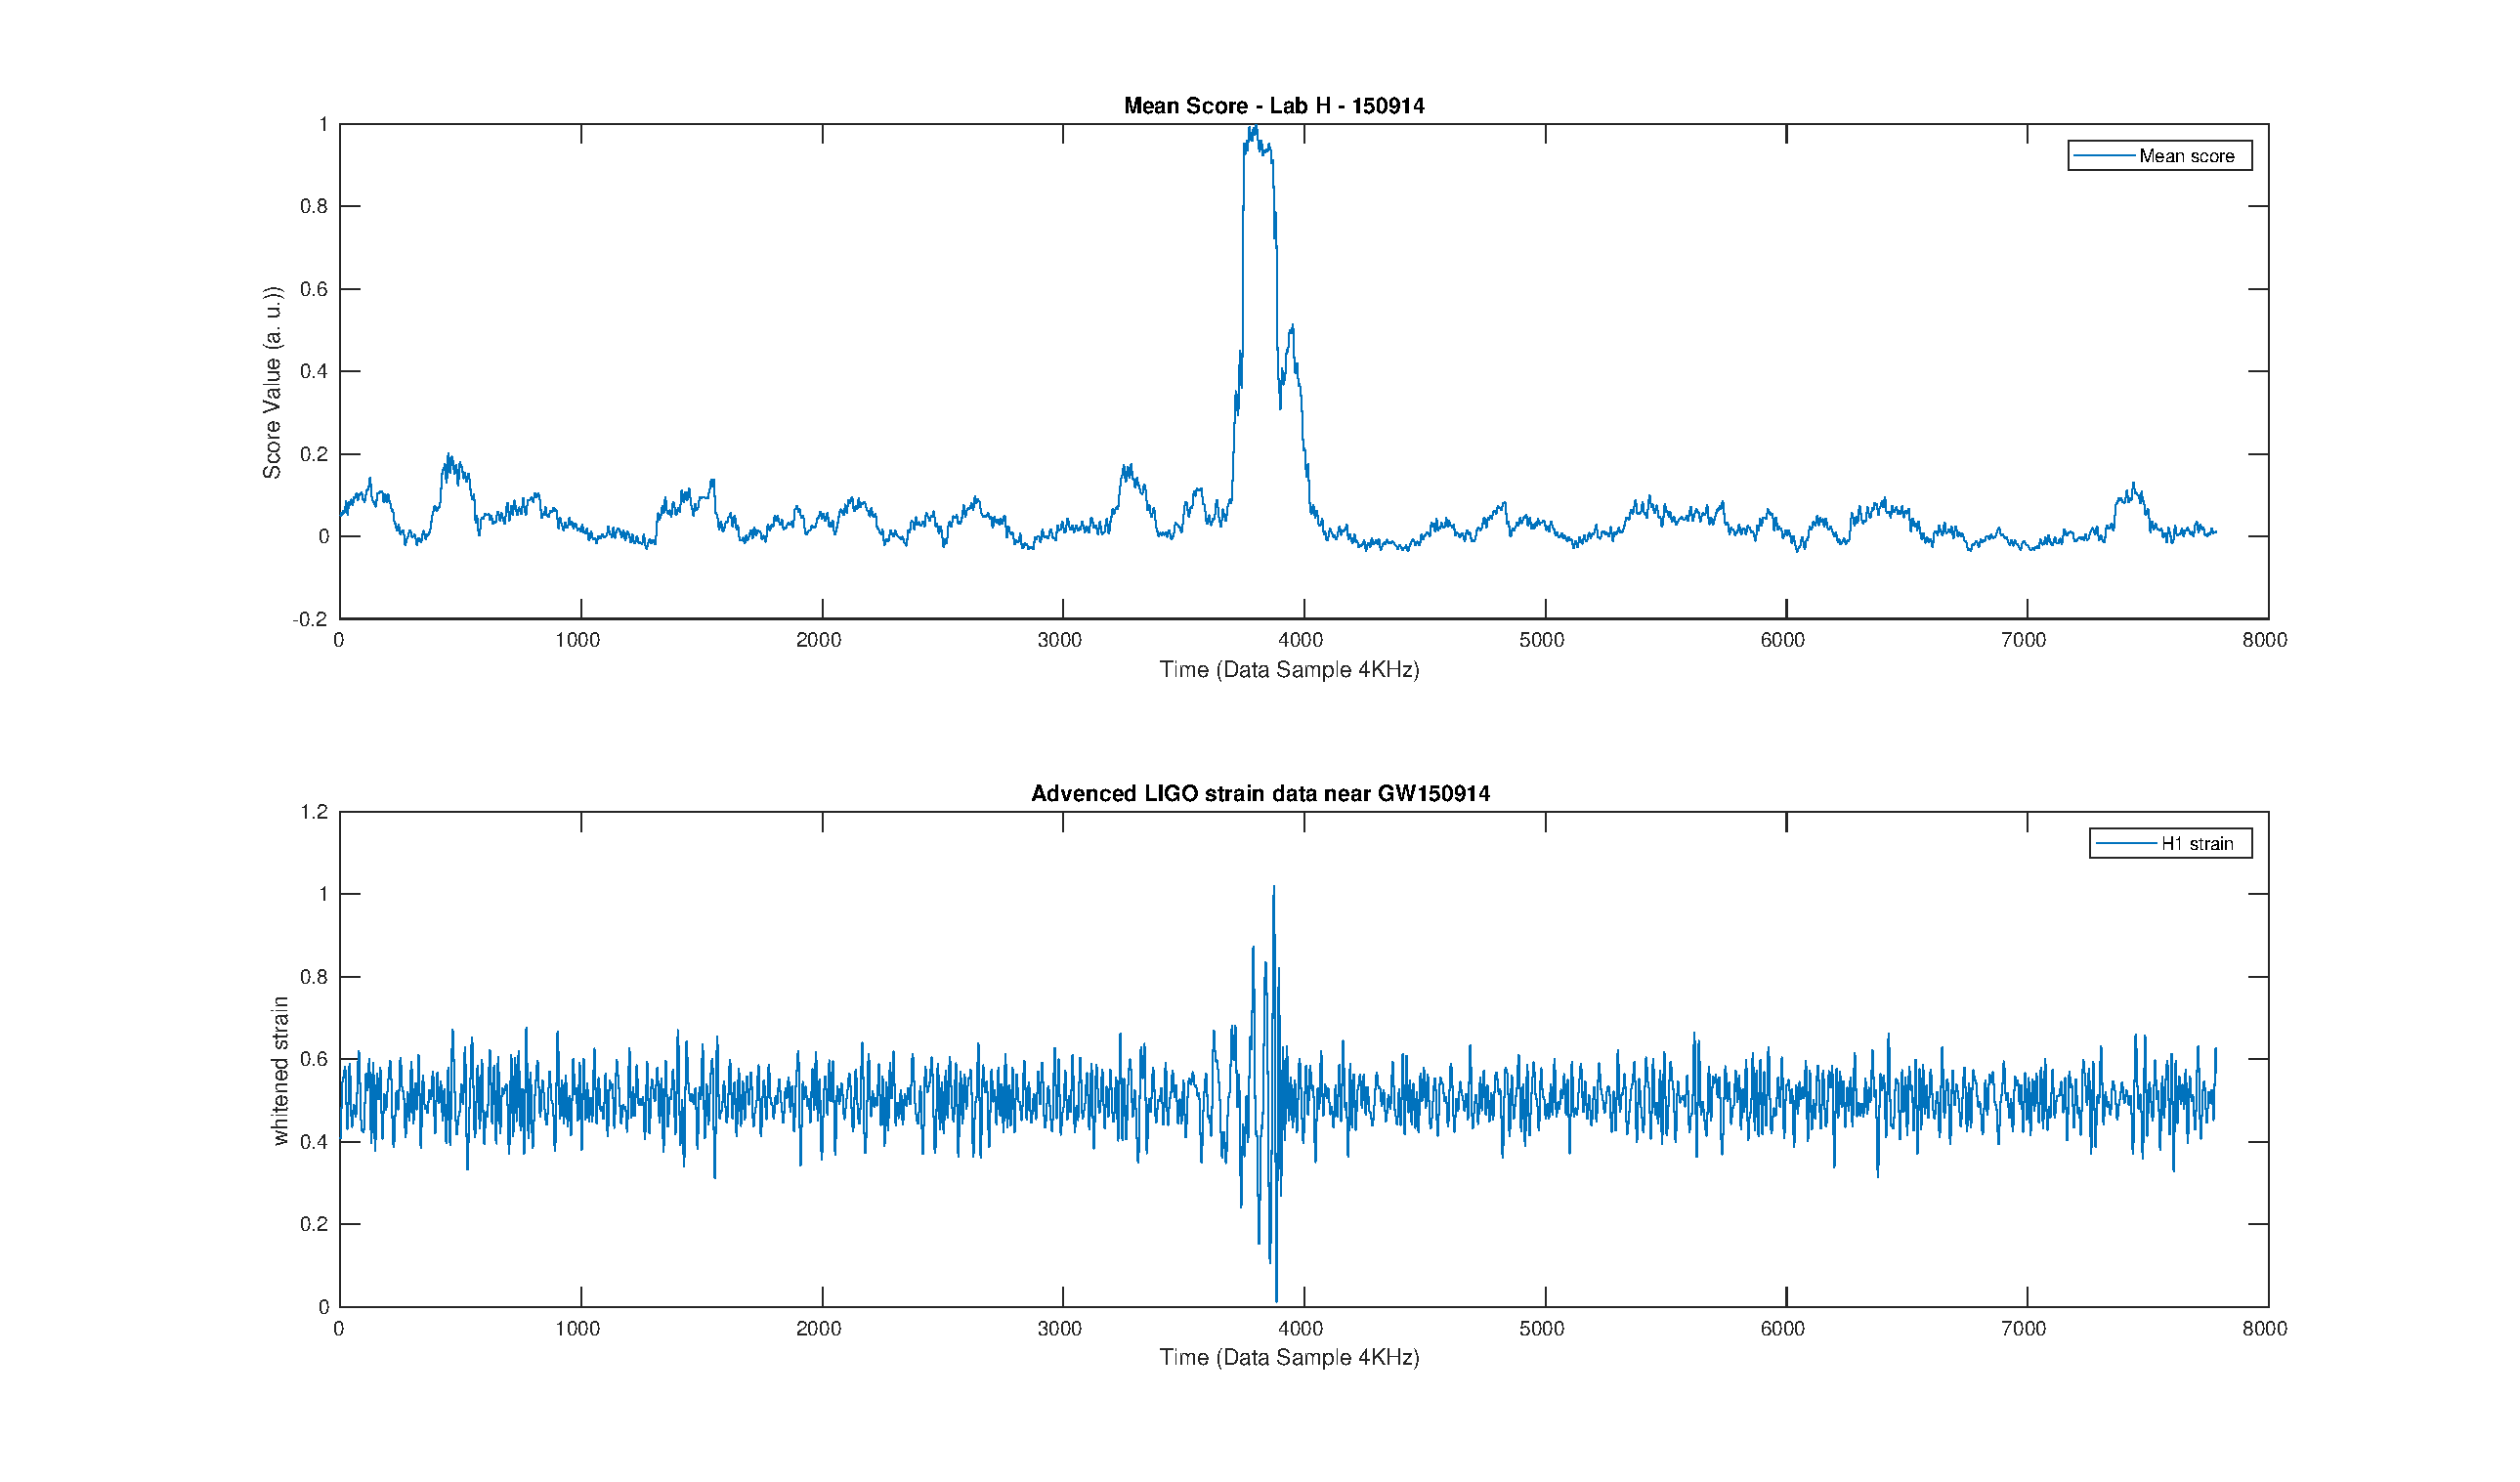
\includegraphics[width=1\textwidth]{figuras/detection.eps}
\caption{Resultado do score do comitê em comparação com os dados de entrada}
\label{fig:detection}
\end{figure}

Assim como o LIGO faz para confirmar a detecção das GW, esta pesquisa adotou a mesma premissa e usou os scores gerados para os dois laboratórios do LIGO, Figura~\ref{fig:score-H1} e~\ref{fig:score-L1} para fazer uma coincidência entre os dados, afim de confirmar a detecção da onda gravitacional.

\begin{figure}[H]
     \centering
     \begin{subfigure}[b]{0.45\textwidth}
         \centering
         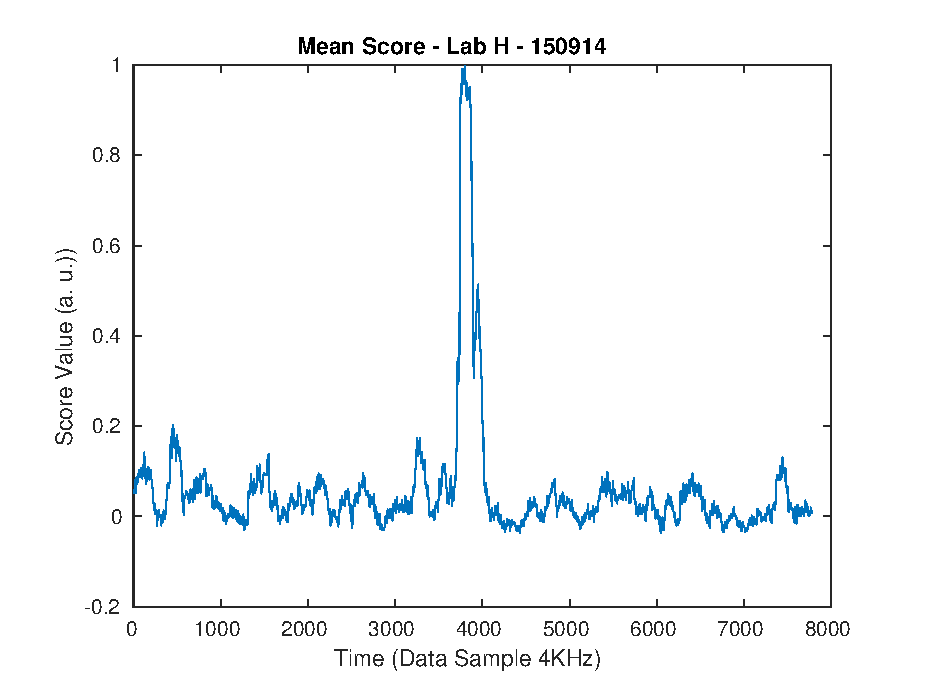
\includegraphics[width=\textwidth]{figuras/GW150914_LabH.eps}
         \caption{Score gerado para o laboratório H}
         \label{fig:score-H1}
     \end{subfigure}
     \hfill
     \begin{subfigure}[b]{0.45\textwidth}
         \centering
         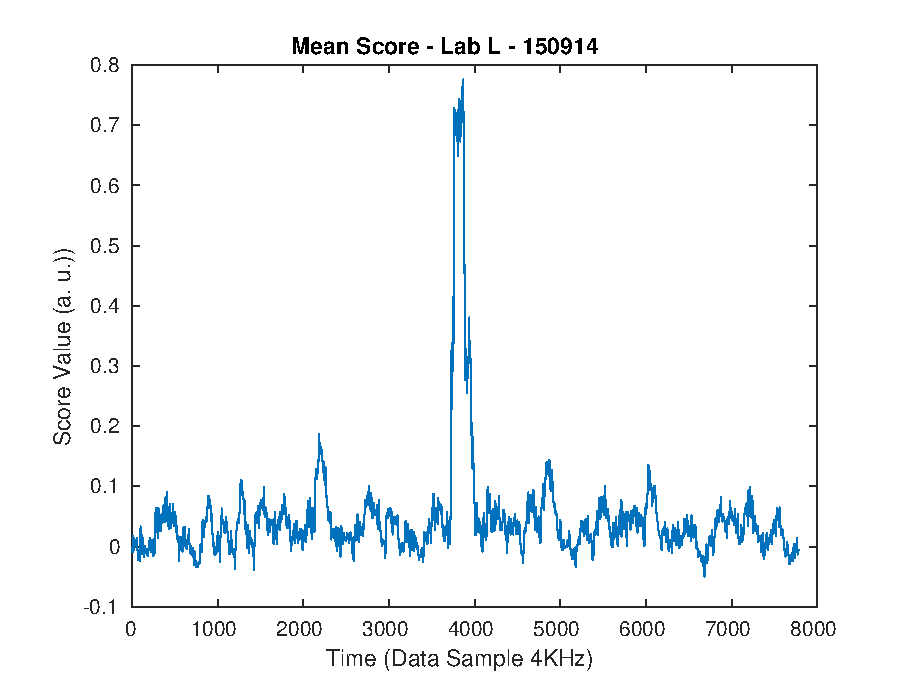
\includegraphics[width=\textwidth]{figuras/GW150914_LabL.eps}
         \caption{Score gerado para o laboratório L}
         \label{fig:score-L1}
     \end{subfigure}
     \caption{Score da onda gravitacional GW150914}
\end{figure}

O resultado desta coincidência de dados gerou um novo score muito mais limpo e claro sobre a detecção da onda gravitacional. É mostrado na Figura~\ref{fig:scoreHL} o resultado da coincidência entre os scores da GW150914 gerados para os dois laboratórios do LIGO.

\begin{figure}[H]
\centering
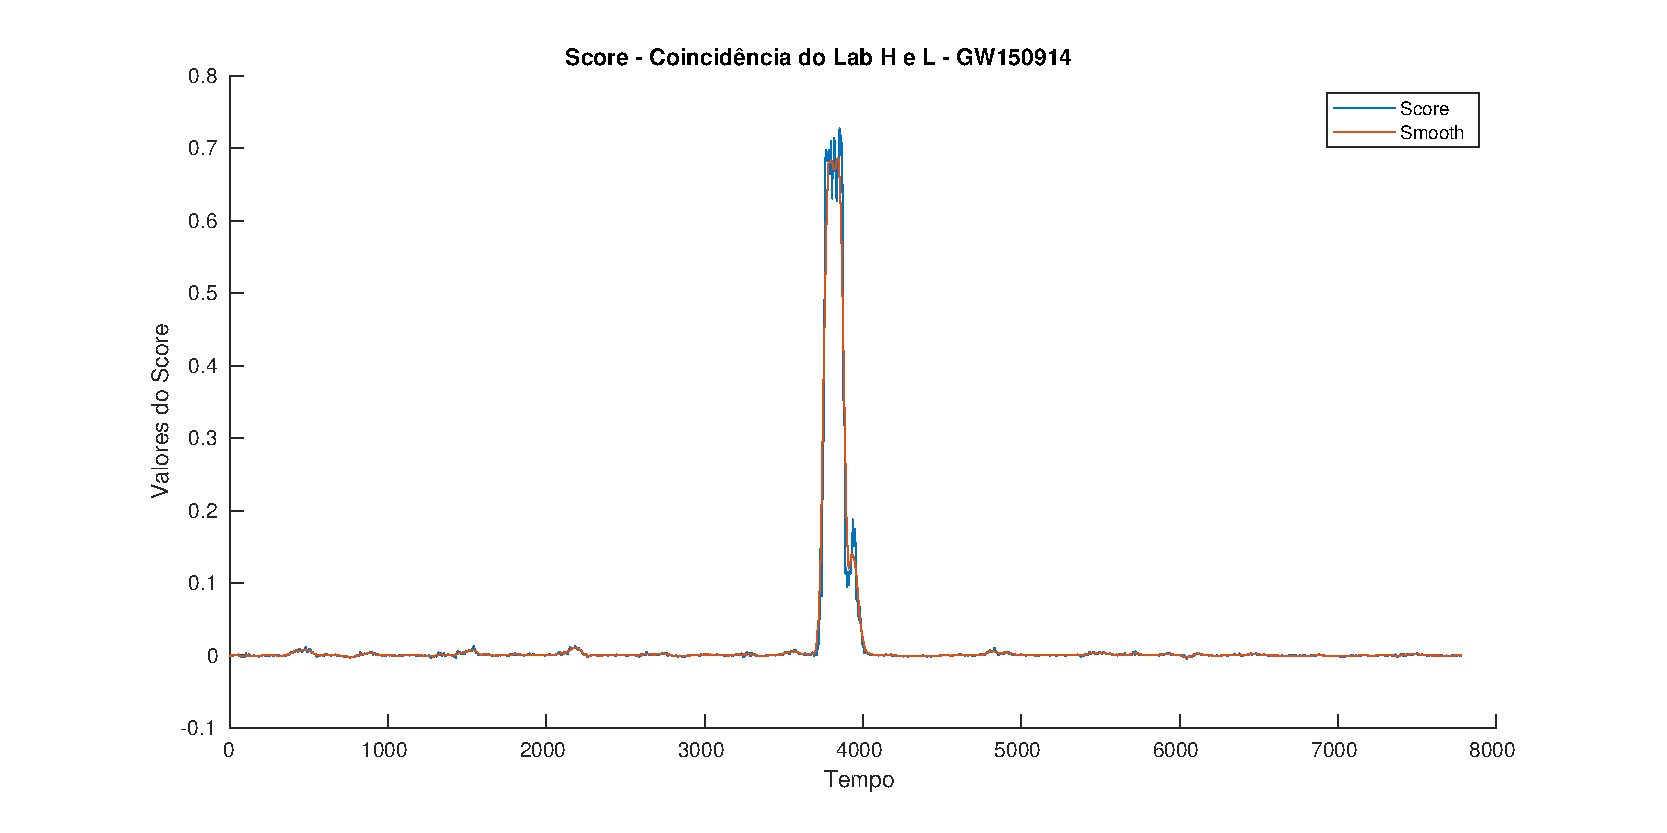
\includegraphics[width=1\textwidth]{figuras/GW150914_LabHL.eps}
\caption{Resultado do score da RNA em comparação com os dados reais do LIGO.}
\label{fig:scoreHL}
\end{figure}

Para uma melhor visualização dos resultados na Figura \ref{fig:scoreHL} é possível notar que foi feito uma suavização dos dados, representada pela linha vermelha (\textit{Smooth}). Nesta Figura \ref{fig:scoreHL} diferente dos resultados individuais de cada laboratório do LIGO, o score não alcança a margem do valor máximo de 1, visto que, apos a coincidência dos dados entre os laboratórios, este valor tende a ficar menor, mas a sua representação permanece em evidencia, o que demostra a detecção da onda gravitacional em meio aos dados. É mostrado na Figura \ref{fig:scoreHLZoom} um zoom deste resultado.

\begin{figure}[H]
\centering
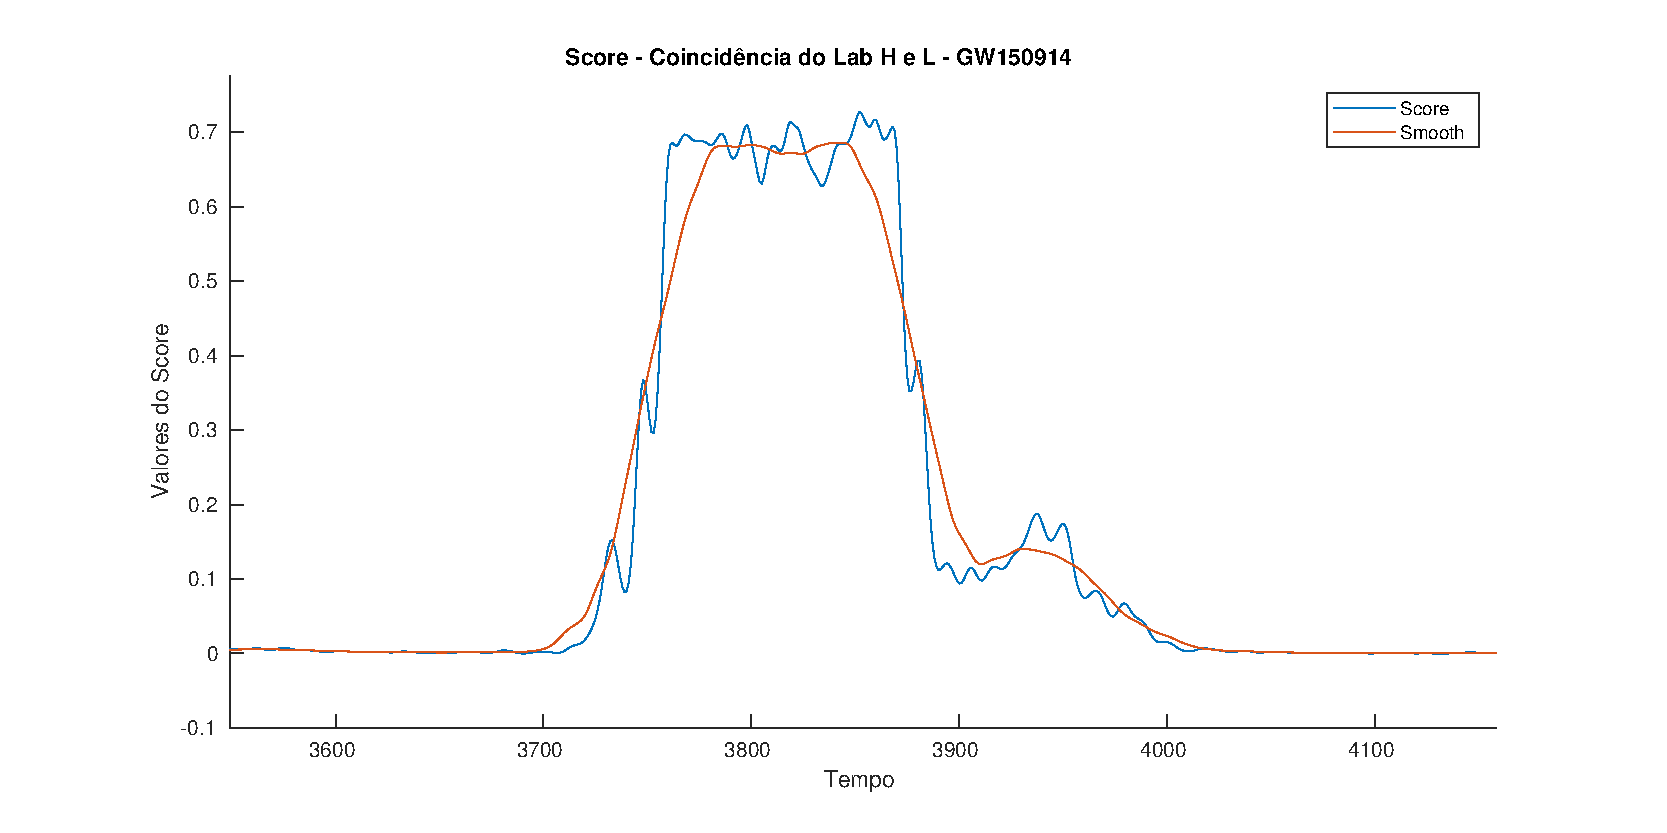
\includegraphics[width=1\textwidth]{figuras/GW150914_LabHL_zoom.eps}
\caption{Zoom do resultado da coincidência entre os laboratórios H1 e L1 para a GW150914.}
\label{fig:scoreHLZoom}
\end{figure}

Além disso, com os resultados é possível apontar a existência de mais informações que podem ser tiradas, como o comportamento da reverberação dos corpos astronômicos após o colapso, a possibilidade de cálculo dos tempos de ringdown, a duração temporal do evento e etc.

Como consequência disto, foi encontrado a estimativa do tempo de fusão-ringdown de todas as GWs usadas nesta pesquisa. Por cauda da complexidade das técnicas de parametrização, até o momento foram descobertas o tempo de ringdown somente em metade das observações feitas pelo LIGO.

Outra grande descoberta inédita, foi a descoberta de um Plator presente em todas os resultados desta pesquisa, é mostrado na Figura \ref{fig:scoreHLPlator} o decaimento do score ao final da fusão dos buracos negros, existe uma pequena ondulação que possivelmente seja a reverberação pós fusão dos dois buracos negros. Estes estudos estão em andamento e serão descritos em um artigo subsequente. 

Diante disto, estas revelações demostram a grande aptidão desta pesquisa em desvendar novas informações sobre as ondas gravitacionais.

\begin{figure}[H]
\centering
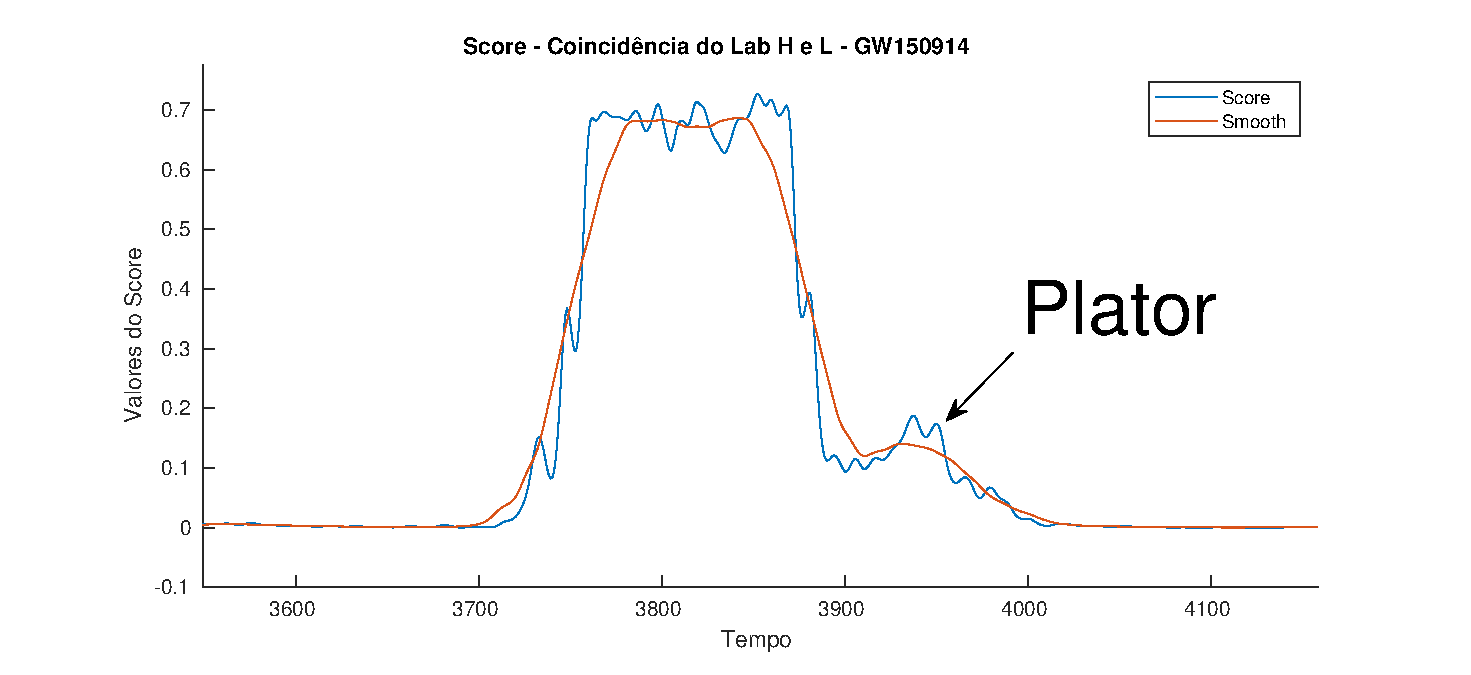
\includegraphics[width=1\textwidth]{figuras/GW150914_LabHL_plator.eps}
\caption{Zoom do resultado da coincidência entre os laboratórios H1 e L1 para a GW150914 com a marcação do Plator.}
\label{fig:scoreHLPlator}
\end{figure}

A possibilidade de encontrar novas informações inéditas sobre as ondas gravitacionais que esta pesquisa trás, a torna um material de pesquisa muito promissor para esta nova areá de pesquisa em ascensão. Além de prover uma ferramenta para auxiliar ou complementar os algoritmos de detecção de ondas gravitacionais existentes.


\chapter{Conclusão}

Desde a confirmação e descoberta das ondas gravitacionais, muito se falou sobre este assunto, consequentemente muitos estudos voltados a esta área vieram a tona. Mesmo assim, poucos estudos foram feitos mesclando o uso de Machine Learning com as ondas gravitacionais. Diante disto, esta pesquisa se caracteriza como uma grande contribuição nesta areá de pesquisa que aos poucos esta atraindo mais visibilidade. 

Nesta pesquisa foi empregado um comitê de redes neurais com hiperparâmetros rigorosamente ajustados e produzido uma saída que retorna uma estatística de classificação equivalente à uma função de pertinência inferida de que os dados contêm um sinal de onda gravitacional, mostrando que o método empregado neste trabalho pode, em princípio, ser usada para pesquisar diretamente sinais GW nos dados, em tempo de pesquisa teoricamente, substancialmente mais rápido do que as abordagens com Deep Learning e filtragem correspondente.

Devido a simplicidade da arquitetura das redes neurais desenvolvidas, torna possível este método capaz de ser reproduzido em ambientes computacionais mais simples, que estão ao alcance do hardware comercial disponível hoje. Além disso, a escalabilidade intrínseca desta metodologia pode superar e abranger o espaço de parâmetros de fusão de buracos negros e ser aplicado a outros tipos de fusão, como sinais de fusão de binários de estrelas de nêutrons e fusão de estrelas de nêutrons com buracos negros. 

Essas capacidades podem permitir pesquisas rápidas e automatizadas de GW em qualquer ambiente, cobrindo milhões ou bilhões de modelos em toda a gama de espaço de parâmetros que está além do alcance dos algoritmos existentes. Portanto, esperamos que essa abordagem aumente a profundidade e a velocidade do algoritmo desenvolvido, permitindo pesquisas online em tempo real após ser treinado com bancos de modelos de milhões ou bilhões de formas de onda.

Os resultados obtidos seguindo a metodologia descrita neste trabalho além de ótimos, abrem um leque de possibilidades de descobertas através deste método. Uma das descobertas preliminares foi a estimativa do tempo de fusão-ringdown de todas as fusões usadas nesta pesquisa, o qual, o LIGO somente tem conhecimento de metade delas. Também foi descoberto um Plator presente em todas os resultados desta pesquisa, na Figura~\ref{fig:scoreHLPlator} é possível notar que após o decaimento do score ao final da fusão dos buracos negros existe uma pequena ondulação que possivelmente pode ser a reverberação pós fusão dos dois buracos negros. Estes estudos estão em andamento e serão descritos em um artigo subsequente. Diante disto, estas revelações demostram a grande aptidão desta pesquisa em desvendar novas informações sobre as ondas gravitacionais.

\begin{figure}[H]
\centering
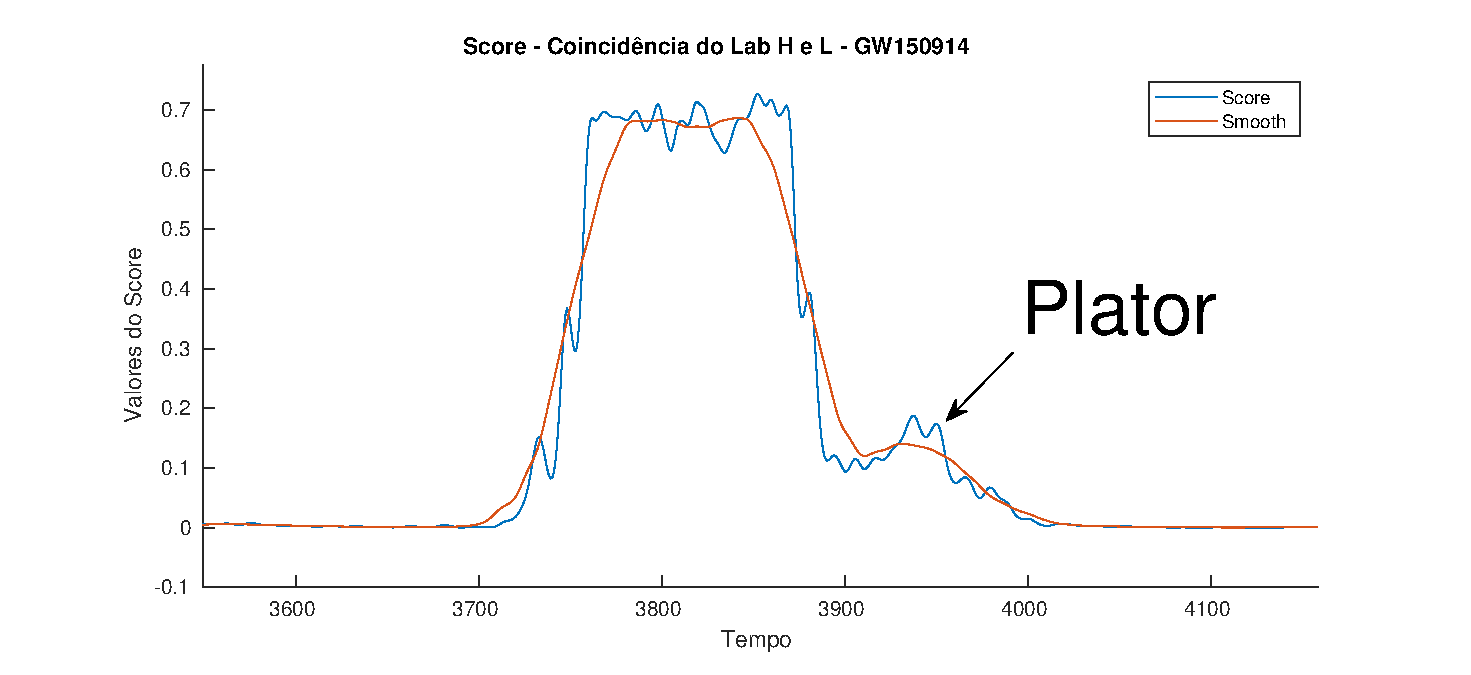
\includegraphics[width=1\textwidth]{figuras/GW150914_LabHL_plator.eps}
\caption{Zoom do resultado da coincidência entre os laboratórios H1 e L1 para a GW150914 com a marcação do Plator.}
\label{fig:scoreHLPlator}
\end{figure}

Além do mais, os resultados apresentados nesta pesquisa fornecem um forte incentivo para estender a metodologia para a possibilidade de estimativa de parâmetros assim como em~\cite{PhysRevD.97.044039,GEORGE201864}. Futuramente, será investido mais esforço no ajuste de hiperparâmetros e inclusão de novas formas de ondas que abrangem diversos parâmetros de fusões, ao ponto de superar a sensibilidade das pesquisas de Deep Learning e matched-filtering. Ademais, será pesquisado a estimação de parâmetros juntamente com a detecção de sinais nos dados do LIGO, tornando a detecção rápida com a estimativa de parâmetros igualmente rápida fundamental para a astronomia de ondas gravitacionais.

Essas considerações fornecem motivação suficiente para desenvolver e implantar novas abordagens nesta área de pesquisa afim de produzir um pipeline de detecção de sinais de GW único, simples e computacionalmente eficiente que unifica a detecção em tempo real de GW e a estimativa de parâmetros, em que, qualquer um posso usar e desenvolver novas pesquisas, fazendo deste um método de pesquisa competitivo.

Esperasse que esta nova abordagem penetre na comunidade científica e sirva como um passo fundamental para permitir observações em tempo real de sinais GW, fornecendo alertas imediatos para acompanhamento após eventos de GW. Também almejasse que esta nova metodologia para processar sinais em dados ruidosos seja útil em muitas outras áreas, tornando essa metodologia muito promissora para vários campos de pesquisa. Fazendo deste trabalho o alicerce para integralizar diversos setores de especialização para permitir e acelerar descobertas científicas.

No geral, esta pesquisa tem potencial para se tornar uma ferramenta útil de pesquisa para a analise de GW, mas há um esforço substancial de pesquisa e desenvolvimento para alcançar isso.


% ----------------------------------------------------------
% ELEMENTOS PÓS-TEXTUAIS
% ----------------------------------------------------------
\postextual
% ----------------------------------------------------------
\chapter{Apêndice A}

aaaaaaaaaaa
% ----------------------------------------------------------
% Referências bibliográficas
% ----------------------------------------------------------
\bibliographystyle{abntex2-alf}
\bibliography{referencias}



%---------------------------------------------------------------------
% INDICE REMISSIVO
%---------------------------------------------------------------------
\phantompart
\printindex

%---------------------------------------------------------------------

\end{document}
